% t-SNE: A Mathematical Journey Through Dimensionality Reduction
% Prof. Endri Raco - Guest Lecture at UPC

\documentclass[10pt]{beamer}
\usetheme{Madrid}
\usecolortheme{seahorse}

% Essential packages only
\usepackage[utf8]{inputenc}
\usepackage{amsmath,amssymb}
\usepackage{graphicx}
\usepackage{tikz}
\usepackage{booktabs}
\usetikzlibrary{shapes.geometric, arrows.meta, positioning, patterns}
\usepackage{algorithm}
\usepackage{algpseudocode}
% Color definitions
\definecolor{upcblue}{RGB}{0,123,199}
\definecolor{upcgray}{RGB}{100,100,100}
\definecolor{highlight}{RGB}{255,127,0}
\definecolor{darkgreen}{RGB}{0,150,0}
\definecolor{darkred}{RGB}{180,0,0}

% Custom commands
\newcommand{\emphtext}[1]{\textcolor{upcblue}{\textbf{#1}}}
\newcommand{\warningbox}[1]{\colorbox{red!10}{\begin{minipage}{0.85\textwidth}\centering #1\end{minipage}}}
\newcommand{\conceptbox}[1]{\colorbox{upcblue!10}{\begin{minipage}{0.85\textwidth}\centering #1\end{minipage}}}

% Slide layout adjustments
\setbeamersize{text margin left=5mm,text margin right=5mm}

\title[t-SNE]{t-Stochastic Neighbor Embedding:\\A Journey from Information Theory to Visualization}
\author[Prof. Raco]{Prof.Asc. Endri Raco\\Polytechnic University of Tirane}
\institute[UPC]{Advanced Multivariate Analysis\\Polytechnic University of Catalonia}
\date{October 15, 2025}

\usepackage{textcomp}
\usepackage{newunicodechar} % Add this package
\newunicodechar{≈}{\ensuremath{\approx}}
\newunicodechar{≠}{\ensuremath{\neq}}
\newunicodechar{≥}{\ensuremath{\geq}}
\newunicodechar{∝}{\ensuremath{\propto}}
\newunicodechar{☐}{\ensuremath{\square}}

\begin{document}



% SLIDE 1: Title
\begin{frame}[plain]
\titlepage
\end{frame}

% SLIDE 2: Learning Objectives
\begin{frame}{What You Will Master Today}
\vspace{-0.2cm}
\begin{columns}[T]
\begin{column}{0.48\textwidth}
\emphtext{Conceptual Understanding}
\begin{itemize}
\footnotesize
\item Information preservation paradigm
\item Maximum entropy principle
\item KL divergence as information waste
\item Crowding problem geometry
\end{itemize}

\vspace{0.3cm}
\emphtext{Mathematical Foundations}
\begin{itemize}
\footnotesize
\item Derive Gaussian kernel from first principles
\item Understand gradient as force system
\item Prove why Student's t solves crowding
\end{itemize}
\end{column}

\begin{column}{0.48\textwidth}
\emphtext{Practical Mastery}
\begin{itemize}
\footnotesize
\item Debug common failures
\item Choose hyperparameters wisely
\item Validate embeddings statistically
\item Avoid interpretation pitfalls
\end{itemize}

\vspace{0.3cm}
\emphtext{Implementation Skills}
\begin{itemize}
\footnotesize
\item Handle numerical stability
\item Optimize for large datasets
\item Compare with modern alternatives
\end{itemize}
\end{column}
\end{columns}

\vspace{0.3cm}
\begin{center}
\warningbox{\footnotesize\textbf{Critical:} We'll integrate mathematics throughout - not as an afterthought, but as the story itself}
\end{center}
\end{frame}

% SLIDE 3: The Central Question
\begin{frame}{The Fundamental Challenge}
\begin{center}
\emphtext{How do we preserve the essence of high-dimensional data\\when forced into 2D for visualization?}
\end{center}

\vspace{0.3cm}
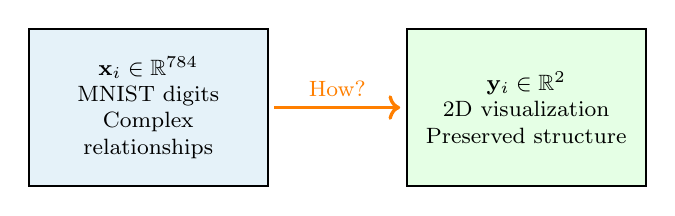
\begin{tikzpicture}[scale=0.8]
% High-D space
\node[draw,thick,minimum width=3cm,minimum height=2cm,fill=upcblue!10] (highd) at (0,0) {
\begin{minipage}{2.8cm}
\centering
\footnotesize
$\mathbf{x}_i \in \mathbb{R}^{784}$\\
MNIST digits\\
Complex relationships
\end{minipage}
};

% Arrow with question
\draw[->,very thick,highlight] (2,0) -- (4,0) node[midway,above] {\footnotesize How?};

% Low-D space  
\node[draw,thick,minimum width=3cm,minimum height=2cm,fill=green!10] (lowd) at (6,0) {
\begin{minipage}{2.8cm}
\centering
\footnotesize
$\mathbf{y}_i \in \mathbb{R}^{2}$\\
2D visualization\\
Preserved structure
\end{minipage}
};
\end{tikzpicture}

\vspace{0.3cm}
\emphtext{The Answer: Preserve Information, Not Distance}

\begin{center}
\conceptbox{
\footnotesize
Traditional methods preserve \textbf{distances} or \textbf{variance}\\
t-SNE preserves \textbf{neighborhood probability distributions}\\
This is the paradigm shift that changes everything
}
\end{center}
\end{frame}

% SLIDE 4: Why Dimensionality Reduction?
\begin{frame}{Why Reduce Dimensions? The Practical Reality}
\begin{columns}[T]
\begin{column}{0.48\textwidth}
\emphtext{The Curse of Dimensionality}

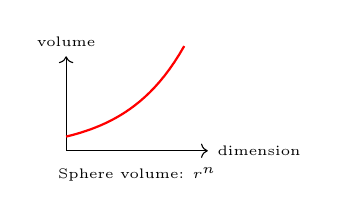
\begin{tikzpicture}[scale=0.6]
\draw[->] (0,0) -- (3,0) node[right] {\tiny dimension};
\draw[->] (0,0) -- (0,2) node[above] {\tiny volume};

% Exponential growth
\draw[thick,red,domain=0:2.5] plot (\x, {0.3*exp(0.8*\x)});
\node at (1.5,-0.5) {\tiny Sphere volume: $r^n$};
\end{tikzpicture}

\footnotesize
\textbf{In 100D:}\\
- 99.99\% of volume in outer shell\\
- All points equidistant\\
- Intuition completely fails
\end{column}

\begin{column}{0.48\textwidth}
\emphtext{Real-World Impact}

\footnotesize
\textbf{Genomics:} 20,000 genes\\
→ Visualize patient clusters

\textbf{NLP:} 50,000 word vocabulary\\
→ See semantic relationships

\textbf{Images:} 1024×1024 pixels\\
→ Discover visual patterns

\vspace{0.2cm}
\textbf{Common thread:}\\
Data lives on low-D manifold\\
in high-D space
\end{column}
\end{columns}

\vspace{0.3cm}
\begin{center}
\warningbox{\footnotesize\textbf{Remember:} We're not just compressing - we're revealing hidden structure}
\end{center}
\end{frame}

% SLIDE 5: Linear Methods Fail
\begin{frame}{Why Linear Methods Fail: The Swiss Roll}
\begin{columns}[T]
\begin{column}{0.48\textwidth}
\emphtext{The Data: 2D Manifold in 3D}

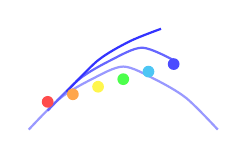
\begin{tikzpicture}[scale=0.8]
% Swiss roll visualization
\draw[thick,blue!40] plot[smooth,tension=0.5] 
    coordinates {(-1.5,0) (-1,0.5) (-0.5,0.8) (0,1) (0.5,0.8) (1,0.5) (1.5,0)};
\draw[thick,blue!60] plot[smooth,tension=0.5]
    coordinates {(-1.2,0.3) (-0.7,0.8) (-0.2,1.1) (0.3,1.3) (0.8,1.1)};
\draw[thick,blue!80] plot[smooth,tension=0.5]
    coordinates {(-0.9,0.6) (-0.4,1.1) (0.1,1.4) (0.6,1.6)};
    
% Color gradient points
\foreach \x/\c in {-1.2/red,-0.8/orange,-0.4/yellow,0/green,0.4/cyan,0.8/blue} {
    \node[circle,fill=\c!70,inner sep=1.5pt] at (\x,{0.8+0.3*\x}) {};
}
\end{tikzpicture}

\footnotesize
True structure: Continuous spiral\\
Neighbors defined by manifold distance
\end{column}

\begin{column}{0.48\textwidth}
\emphtext{PCA Projection Fails}

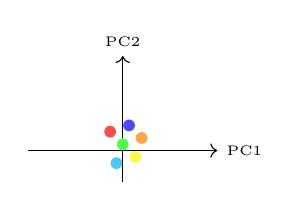
\begin{tikzpicture}[scale=0.8]
% Axes
\draw[->] (-1.5,0) -- (1.5,0) node[right] {\tiny PC1};
\draw[->] (0,-0.5) -- (0,1.5) node[above] {\tiny PC2};

% Mixed up points - PCA failure
\node[circle,fill=red!70,inner sep=1.5pt] at (-0.2,0.3) {};
\node[circle,fill=blue!70,inner sep=1.5pt] at (0.1,0.4) {};
\node[circle,fill=orange!70,inner sep=1.5pt] at (0.3,0.2) {};
\node[circle,fill=cyan!70,inner sep=1.5pt] at (-0.1,-0.2) {};
\node[circle,fill=yellow!70,inner sep=1.5pt] at (0.2,-0.1) {};
\node[circle,fill=green!70,inner sep=1.5pt] at (0,0.1) {};
\end{tikzpicture}

\footnotesize
\textcolor{darkred}{Neighbors torn apart!}\\
Linear projection preserves variance\\
but destroys local relationships
\end{column}
\end{columns}

\vspace{0.3cm}
\begin{center}
\conceptbox{\footnotesize\textbf{Key Insight:} We need nonlinear methods that respect local geometry}
\end{center}
\end{frame}

% SLIDE 6: The Information Perspective
\begin{frame}{Reframing the Problem: Information Theory}
\emphtext{The Paradigm Shift: From Distances to Information}

\vspace{0.3cm}
\begin{center}
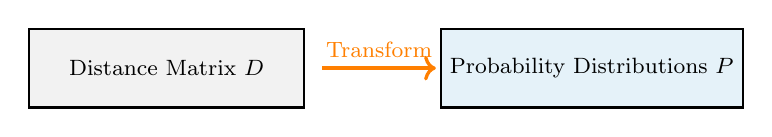
\begin{tikzpicture}[scale=0.9]
% Old way
\node[draw,thick,fill=gray!10,minimum width=3.5cm,minimum height=1cm] at (-3,0) {
\footnotesize Distance Matrix $D$
};

% New way
\node[draw,thick,fill=upcblue!10,minimum width=3.5cm,minimum height=1cm] at (3,0) {
\footnotesize Probability Distributions $P$
};

% Arrow
\draw[->,very thick,highlight] (-0.8,0) -- (0.8,0) node[midway,above] {\footnotesize Transform};
\end{tikzpicture}
\end{center}

\vspace{0.3cm}
\emphtext{Information Content of a Neighborhood:}

If point $j$ has probability $p_{j|i}$ of being $i$'s neighbor:
$$I(j) = -\log p_{j|i} \text{ bits}$$

Total information about $i$'s neighborhood:
$$H(P_i) = -\sum_j p_{j|i} \log p_{j|i} \text{ bits (entropy)}$$

\vspace{0.2cm}
\begin{center}
\warningbox{\footnotesize\textbf{Critical Question:} How much information is lost when we map to 2D?}
\end{center}

This is what t-SNE minimizes!
\end{frame}

% SLIDE 7: Building Probabilities - Part 1
\begin{frame}{From Distances to Probabilities: Step by Step}
\emphtext{The Challenge: Define "Neighborhood" Adaptively}

\vspace{0.3cm}
\begin{columns}[T]
\begin{column}{0.48\textwidth}
\textbf{Dense Region}
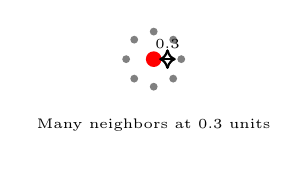
\begin{tikzpicture}[scale=0.7]
\node[circle,fill=red,inner sep=2pt] (c) at (0,0) {};
\foreach \angle in {0,45,90,135,180,225,270,315} {
    \node[circle,fill=gray,inner sep=1pt] at ({0.5*cos(\angle)},{0.5*sin(\angle)}) {};
}
\draw[<->,thick] (0.1,0) -- (0.4,0) node[midway,above] {\tiny 0.3};
\node at (0,-1.2) {\tiny Many neighbors at 0.3 units};
\end{tikzpicture}
\end{column}

\begin{column}{0.48\textwidth}
\textbf{Sparse Region}
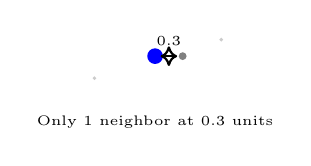
\begin{tikzpicture}[scale=0.7]
\node[circle,fill=blue,inner sep=2pt] (c) at (0,0) {};
\node[circle,fill=gray,inner sep=1pt] at (0.5,0) {};
\node[circle,fill=gray!40,inner sep=0.5pt] at (1.2,0.3) {};
\node[circle,fill=gray!40,inner sep=0.5pt] at (-1.1,-0.4) {};
\draw[<->,thick] (0.1,0) -- (0.4,0) node[midway,above] {\tiny 0.3};
\node at (0,-1.2) {\tiny Only 1 neighbor at 0.3 units};
\end{tikzpicture}
\end{column}
\end{columns}

\vspace{0.3cm}
\emphtext{Solution: Adaptive Gaussian Kernel}

\begin{center}
\conceptbox{
$$\text{similarity}_{j|i} = \exp\left(-\frac{\|\mathbf{x}_i - \mathbf{x}_j\|^2}{2\sigma_i^2}\right)$$
\footnotesize $\sigma_i$ adapts to local density!
}
\end{center}

But why this specific form? Let's derive it...
\end{frame}

% SLIDE 8: Maximum Entropy Derivation
\begin{frame}{Why Gaussian? The Maximum Entropy Principle}
\emphtext{Deriving the Kernel from First Principles}

\vspace{0.2cm}
\textbf{Given constraints, choose the least biased distribution:}

Maximize entropy: $H(P_i) = -\sum_j p_{j|i} \log p_{j|i}$

Subject to:
\begin{align}
\sum_j p_{j|i} &= 1 \quad \text{(probability)}\\
\sum_j p_{j|i} d_{ij}^2 &= \sigma_i^2 \quad \text{(expected distance)}
\end{align}

\textbf{Lagrangian:}
$$\mathcal{L} = H(P_i) + \lambda(\sum_j p_{j|i} - 1) + \mu(\sum_j p_{j|i} d_{ij}^2 - \sigma_i^2)$$

\textbf{Solution:} $\frac{\partial \mathcal{L}}{\partial p_{j|i}} = 0$ gives:

\begin{center}
\colorbox{green!10}{
\begin{minipage}{0.7\textwidth}
\centering
$$p_{j|i} = \frac{\exp(-d_{ij}^2/2\sigma_i^2)}{\sum_k \exp(-d_{ik}^2/2\sigma_i^2)}$$
\end{minipage}
}
\end{center}

\footnotesize
\textit{The Gaussian emerges naturally - it's not arbitrary!}
\end{frame}

% SLIDE 9: Perplexity as Information
\begin{frame}{Perplexity: The Effective Number of Neighbors}
\emphtext{From $\sigma_i$ to an Intuitive Parameter}

\vspace{0.3cm}
\textbf{Problem:} How to set $\sigma_i$ for thousands of points?

\textbf{Solution:} Specify "effective neighbors" instead!

\vspace{0.2cm}
\begin{columns}[T]
\begin{column}{0.48\textwidth}
\textbf{Perplexity Definition:}
$$\text{Perp}(P_i) = 2^{H(P_i)}$$

\footnotesize
Interpretation:\\
- Uniform over 30 points → Perp = 30\\
- Concentrated on 5 points → Perp ≈ 5\\
- Spread over 100 points → Perp varies
\end{column}

\begin{column}{0.48\textwidth}
\textbf{Finding $\sigma_i$:}
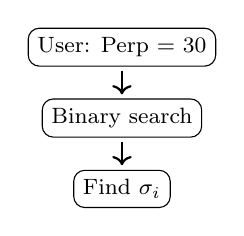
\begin{tikzpicture}[scale=0.6]
\node[draw,rounded corners] at (0,0) {\footnotesize User: Perp = 30};
\draw[->,thick] (0,-0.5) -- (0,-1);
\node[draw,rounded corners] at (0,-1.5) {\footnotesize Binary search};
\draw[->,thick] (0,-2) -- (0,-2.5);
\node[draw,rounded corners] at (0,-3) {\footnotesize Find $\sigma_i$};
\end{tikzpicture}

\footnotesize
Automatic adaptation to density!
\end{column}
\end{columns}

\vspace{0.3cm}
\begin{center}
\warningbox{\footnotesize\textbf{Implementation:} Typical perplexity: 5-50. Must be < n/3}
\end{center}
\end{frame}

% SLIDE 10: KL Divergence Intuition
\begin{frame}{Measuring Information Loss: KL Divergence}
\emphtext{How Wrong Is Our Map?}

\vspace{0.3cm}
\textbf{Cross-Entropy:} Bits needed using wrong distribution Q
$$H(P,Q) = -\sum_j p_j \log q_j$$

\textbf{KL Divergence:} Extra bits due to using Q instead of P
$$\text{KL}(P||Q) = H(P,Q) - H(P) = \sum_j p_j \log\frac{p_j}{q_j}$$

\vspace{0.3cm}
\emphtext{Critical Asymmetry:}

\begin{center}
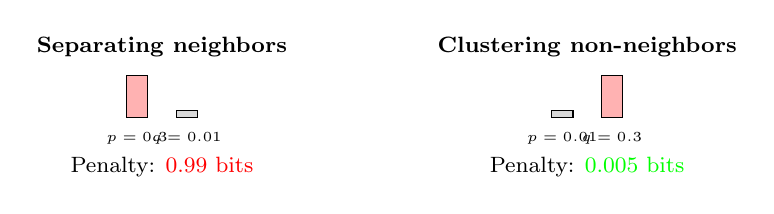
\begin{tikzpicture}[scale=0.9]
% Case 1
\node at (-3,1) {\footnotesize \textbf{Separating neighbors}};
\draw[fill=red!30] (-3.5,0) rectangle (-3.2,0.6);
\draw[fill=gray!30] (-2.8,0) rectangle (-2.5,0.1);
\node at (-3.35,-0.3) {\tiny $p=0.3$};
\node at (-2.65,-0.3) {\tiny $q=0.01$};
\node at (-3,-0.7) {\footnotesize Penalty: \textcolor{red}{0.99 bits}};

% Case 2  
\node at (3,1) {\footnotesize \textbf{Clustering non-neighbors}};
\draw[fill=gray!30] (2.5,0) rectangle (2.8,0.1);
\draw[fill=red!30] (3.2,0) rectangle (3.5,0.6);
\node at (2.65,-0.3) {\tiny $p=0.01$};
\node at (3.35,-0.3) {\tiny $q=0.3$};
\node at (3,-0.7) {\footnotesize Penalty: \textcolor{green}{0.005 bits}};
\end{tikzpicture}
\end{center}

\begin{center}
\conceptbox{\footnotesize t-SNE is obsessed with preserving neighborhoods!}
\end{center}
\end{frame}

% SLIDE 11: The SNE Algorithm
\begin{frame}{The Original SNE Algorithm}
\emphtext{Putting It Together}

\vspace{0.3cm}
\begin{columns}[T]
\begin{column}{0.48\textwidth}
\textbf{High-D Similarities:}
$$p_{j|i} = \frac{e^{-\|\mathbf{x}_i-\mathbf{x}_j\|^2/2\sigma_i^2}}{\sum_k e^{-\|\mathbf{x}_i-\mathbf{x}_k\|^2/2\sigma_i^2}}$$

\textbf{Low-D Similarities:}
$$q_{j|i} = \frac{e^{-\|\mathbf{y}_i-\mathbf{y}_j\|^2}}{\sum_k e^{-\|\mathbf{y}_i-\mathbf{y}_k\|^2}}$$

\footnotesize Note: Fixed variance in low-D!
\end{column}

\begin{column}{0.48\textwidth}
\textbf{Cost Function:}
$$C = \sum_i \text{KL}(P_i||Q_i)$$

\textbf{Optimization:}
$$\mathbf{y}_i \leftarrow \mathbf{y}_i - \eta \frac{\partial C}{\partial \mathbf{y}_i}$$

\footnotesize
Gradient = sum of forces\\
from all other points
\end{column}
\end{columns}

\vspace{0.3cm}
\begin{center}
\warningbox{\footnotesize\textbf{Fatal Flaw:} The Crowding Problem - let's see why...}
\end{center}
\end{frame}

% SLIDE 12: The Crowding Problem
\begin{frame}{SNE's Fatal Flaw: The Crowding Problem}
\emphtext{A Geometric Disaster}

\vspace{0.3cm}
\begin{columns}[T]
\begin{column}{0.48\textwidth}
\textbf{Volume in n-D Spheres:}

Shell from radius 0.9 to 1.0:
\begin{itemize}
\footnotesize
\item 2D: 19\% of area
\item 10D: 65\% of volume  
\item 100D: 99.997\% of volume!
\end{itemize}

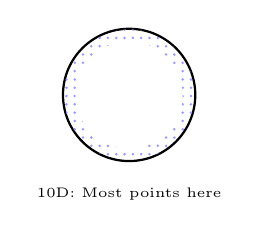
\begin{tikzpicture}[scale=0.7]
\draw[thick] (0,0) circle (1.2cm);
\draw[pattern=dots,pattern color=blue!40] (0,0) circle (1.2cm);
\draw[white,fill=white] (0,0) circle (0.96cm);
\node at (0,-1.8) {\tiny 10D: Most points here};
\end{tikzpicture}
\end{column}

\begin{column}{0.48\textwidth}
\textbf{The Disaster:}

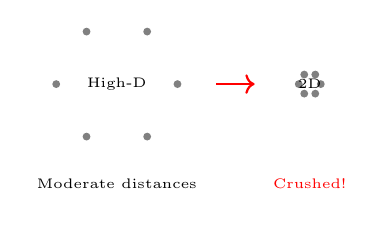
\begin{tikzpicture}[scale=0.7]
% High-D moderate distances
\foreach \angle in {0,60,120,180,240,300} {
    \node[circle,fill=gray,inner sep=1pt] at ({1.1*cos(\angle)},{1.1*sin(\angle)}) {};
}
\node at (0,0) {\tiny High-D};
\node at (0,-1.8) {\tiny Moderate distances};

% Arrow
\draw[->,thick,red] (1.8,0) -- (2.5,0);

% Low-D crushed
\foreach \angle in {0,60,120,180,240,300} {
    \node[circle,fill=gray,inner sep=1pt] at ({3.5+0.2*cos(\angle)},{0.2*sin(\angle)}) {};
}
\node at (3.5,0) {\tiny 2D};
\node at (3.5,-1.8) {\tiny \textcolor{red}{Crushed!}};
\end{tikzpicture}

\footnotesize
Can't represent moderate\\
distances in 2D with Gaussian!
\end{column}
\end{columns}

\vspace{0.3cm}
\begin{center}
\conceptbox{\footnotesize\textbf{Solution:} Use a distribution with heavier tails in low-D!}
\end{center}
\end{frame}

% SLIDE 13: Enter t-SNE
\begin{frame}{The t-SNE Innovation: Heavy Tails}
\emphtext{Van der Maaten \& Hinton's Brilliant Solution (2008)}

\vspace{0.3cm}
\begin{center}
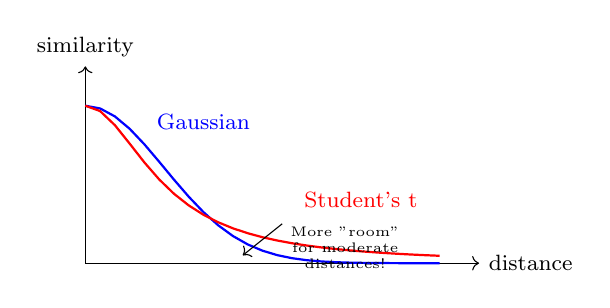
\begin{tikzpicture}[scale=1.0]
\draw[->] (0,0) -- (5,0) node[right] {\footnotesize distance};
\draw[->] (0,0) -- (0,2.5) node[above] {\footnotesize similarity};

% Gaussian
\draw[thick,blue,domain=0:4.5] plot (\x, {2*exp(-0.5*\x*\x)});
\node[blue] at (1.5,1.8) {\footnotesize Gaussian};

% Student's t
\draw[thick,red,domain=0:4.5] plot (\x, {2/(1+\x*\x)});
\node[red] at (3.5,0.8) {\footnotesize Student's t};

% Annotations
\draw[<-] (2,0.1) -- (2.5,0.5);
\node at (3.3,0.4) {\tiny More "room"};
\node at (3.3,0.2) {\tiny for moderate};
\node at (3.3,0) {\tiny distances!};
\end{tikzpicture}
\end{center}

\vspace{0.2cm}
\textbf{Mathematical Form:}
\begin{columns}[T]
\begin{column}{0.48\textwidth}
\footnotesize
High-D (unchanged):
$$p_{ij} \propto e^{-d_{ij}^2}$$
\end{column}
\begin{column}{0.48\textwidth}
\footnotesize
Low-D (NEW):
$$q_{ij} \propto (1+d_{ij}^2)^{-1}$$
\end{column}
\end{columns}

\vspace{0.3cm}
\begin{center}
\warningbox{\footnotesize\textbf{Key:} Polynomial decay vs exponential decay}
\end{center}
\end{frame}

% SLIDE 14: Why It Works Mathematically
\begin{frame}{Why Student's t Solves Crowding: The Math}
\emphtext{Quantifying the Solution}

\vspace{0.3cm}
\textbf{Ratio of Similarities at Different Distances:}

For distances $d_1 = 1$ and $d_2 = 3$:

\begin{columns}[T]
\begin{column}{0.48\textwidth}
\textbf{Gaussian:}
$$\frac{q(d_1)}{q(d_2)} = \frac{e^{-1}}{e^{-9}} = e^8 \approx 2981$$

\footnotesize
Moderate distance effectively\\
becomes "infinite"
\end{column}

\begin{column}{0.48\textwidth}
\textbf{Student's t:}
$$\frac{q(d_1)}{q(d_2)} = \frac{1/(1+1)}{1/(1+9)} = 5$$

\footnotesize
Moderate distance remains\\
meaningfully different
\end{column}
\end{columns}

\vspace{0.3cm}
\emphtext{Effective Volume Created:}

\begin{center}
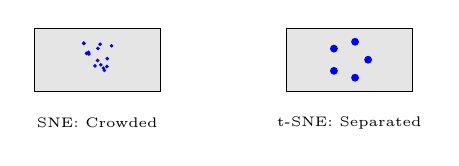
\begin{tikzpicture}[scale=0.8]
% Before (SNE)
\draw[fill=gray!20] (-3,-0.5) rectangle (-1,0.5);
\foreach \i in {1,...,15} {
    \pgfmathsetmacro{\rx}{0.3*rand}
    \pgfmathsetmacro{\ry}{0.3*rand}
    \node[circle,fill=blue,inner sep=0.5pt] at (-2+\rx,\ry) {};
}
\node at (-2,-1) {\tiny SNE: Crowded};

% After (t-SNE)
\draw[fill=gray!20] (1,-0.5) rectangle (3,0.5);
\foreach \angle in {0,72,144,216,288} {
    \node[circle,fill=blue,inner sep=1pt] at ({2+0.3*cos(\angle)},{0.3*sin(\angle)}) {};
}
\node at (2,-1) {\tiny t-SNE: Separated};
\end{tikzpicture}
\end{center}
\end{frame}

% SLIDE 15: The t-SNE Gradient
\begin{frame}{The t-SNE Gradient: Mathematical Elegance}
\emphtext{A Remarkably Clean Form}

\vspace{0.3cm}
With Student's t kernel, the gradient becomes:

\begin{center}
\colorbox{upcblue!10}{
\begin{minipage}{0.85\textwidth}
\centering
$$\frac{\partial C}{\partial \mathbf{y}_i} = 4\sum_j (p_{ij} - q_{ij})(\mathbf{y}_i - \mathbf{y}_j)(1 + \|\mathbf{y}_i - \mathbf{y}_j\|^2)^{-1}$$
\end{minipage}
}
\end{center}

\vspace{0.3cm}
\textbf{Interpreting Each Component:}

\begin{center}
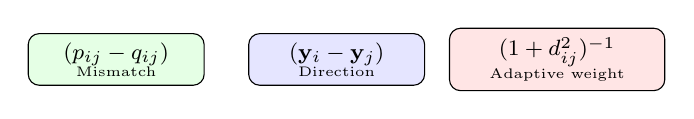
\begin{tikzpicture}[scale=0.8]
\node[draw,rounded corners,fill=green!10] at (-3.5,0) {
\begin{minipage}{2cm}
\centering
\footnotesize $(p_{ij} - q_{ij})$\\
\tiny Mismatch
\end{minipage}
};

\node[draw,rounded corners,fill=blue!10] at (0,0) {
\begin{minipage}{2cm}
\centering
\footnotesize $(\mathbf{y}_i - \mathbf{y}_j)$\\
\tiny Direction
\end{minipage}
};

\node[draw,rounded corners,fill=red!10] at (3.5,0) {
\begin{minipage}{2.5cm}
\centering
\footnotesize $(1 + d_{ij}^2)^{-1}$\\
\tiny Adaptive weight
\end{minipage}
};
\end{tikzpicture}
\end{center}

\vspace{0.2cm}
\emphtext{Key Insight:} The $(1+d_{ij}^2)^{-1}$ term naturally dampens forces\\
between distant points - preventing distant clusters from merging!
\end{frame}

% SLIDE 16: Implementation Reality
\begin{frame}{Implementation: What Really Happens}
\emphtext{From Theory to Practice}

\vspace{0.3cm}
\begin{columns}[T]
\begin{column}{0.48\textwidth}
\textbf{Computational Reality:}
\footnotesize
\begin{tabular}{lr}
\toprule
Dataset Size & Runtime \\
\midrule
1,000 points & 15 seconds \\
10,000 points & 2 minutes \\
100,000 points & 45 minutes \\
1,000,000 points & 8 hours \\
\bottomrule
\end{tabular}

\vspace{0.2cm}
\textit{(Barnes-Hut, 1000 iterations)}
\end{column}

\begin{column}{0.48\textwidth}
\textbf{Memory Requirements:}
\footnotesize
\begin{tabular}{lr}
\toprule
Component & Memory \\
\midrule
Distance matrix & $O(n^2)$ \\
P matrix & $O(n^2)$ \\
Barnes-Hut tree & $O(n\log n)$ \\
Gradient & $O(n)$ \\
\bottomrule
\end{tabular}

\vspace{0.2cm}
\textit{Use sparse P for large n!}
\end{column}
\end{columns}

\vspace{0.3cm}
\textbf{Numerical Stability Fixes:}
\begin{itemize}
\footnotesize
\item Add $\epsilon = 10^{-12}$ to denominators
\item Use log-sum-exp trick for softmax
\item Clip gradients if $\|\nabla\| > 100$
\end{itemize}

\begin{center}
\warningbox{\footnotesize\textbf{Critical:} Always check for NaN/Inf in similarities!}
\end{center}
\end{frame}

% SLIDE 17: Optimization Tricks
\begin{frame}{Making t-SNE Work: Optimization Tricks}
\emphtext{Engineering for Success}

\vspace{0.3cm}
\textbf{1. Early Exaggeration (First 250 iterations):}
\begin{center}
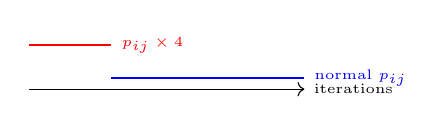
\begin{tikzpicture}[scale=0.7]
\draw[->] (0,0) -- (5,0) node[right] {\tiny iterations};
\draw[thick,red] (0,0.8) -- (1.5,0.8) node[right] {\tiny $p_{ij} \times 4$};
\draw[thick,blue] (1.5,0.2) -- (5,0.2) node[right] {\tiny normal $p_{ij}$};
\end{tikzpicture}
\end{center}
\footnotesize Effect: Forms tight clusters early

\vspace{0.2cm}
\textbf{2. Momentum Schedule:}
$$v^{(t+1)} = \alpha(t) v^{(t)} + \eta \nabla C$$
\footnotesize
$\alpha = 0.5$ (early) → $\alpha = 0.8$ (after iteration 250)

\vspace{0.2cm}
\textbf{3. Adaptive Learning Rate:}
\footnotesize
\begin{itemize}
\item If $\text{sign}(\nabla^{(t)}) = \text{sign}(\nabla^{(t-1)})$: $\eta \times 1.2$
\item If $\text{sign}(\nabla^{(t)}) \neq \text{sign}(\nabla^{(t-1)})$: $\eta \times 0.8$
\item Min: 10, Max: 1000
\end{itemize}

\begin{center}
\conceptbox{\footnotesize These tricks reduce convergence time by 5-10×!}
\end{center}
\end{frame}

% SLIDE 18: Barnes-Hut Acceleration
\begin{frame}{Barnes-Hut: From $O(n^2)$ to $O(n\log n)$}
\emphtext{Making t-SNE Scalable}

\vspace{0.3cm}
\textbf{Key Observation:} Most computation is repulsive forces

\begin{columns}[T]
\begin{column}{0.48\textwidth}
\textbf{The Idea:}
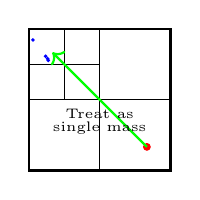
\begin{tikzpicture}[scale=0.6]
% Quadtree
\draw[thick] (0,0) rectangle (3,3);
\draw (1.5,0) -- (1.5,3);
\draw (0,1.5) -- (3,1.5);
\draw (0.75,1.5) -- (0.75,3);
\draw (0,2.25) -- (1.5,2.25);

% Points
\foreach \i in {1,...,4} {
    \node[circle,fill=blue,inner sep=0.5pt] at ({0.3+0.3*rand},{2.5+0.3*rand}) {};
}
\node[circle,fill=red,inner sep=1pt] at (2.5,0.5) {};

% Arrow showing approximation
\draw[->,thick,green] (2.5,0.5) -- (0.5,2.5);
\node at (1.5,1.2) {\tiny Treat as};
\node at (1.5,0.9) {\tiny single mass};
\end{tikzpicture}
\end{column}

\begin{column}{0.48\textwidth}
\textbf{Criterion:}
$$\frac{r_{\text{cell}}}{d_{\text{to cell}}} < \theta$$

\footnotesize
$\theta = 0.5$: Good balance\\
$\theta = 0$: Exact (slow)\\
$\theta = 1$: Fast (inaccurate)

\vspace{0.2cm}
\textbf{Speedup:}\\
10K points: 50× faster\\
100K points: 200× faster
\end{column}
\end{columns}

\vspace{0.3cm}
\begin{center}
\warningbox{\footnotesize\textbf{Trade-off:} 1-2\% accuracy loss for massive speedup}
\end{center}
\end{frame}

% SLIDE 19: Debugging t-SNE
\begin{frame}{Debugging t-SNE: A Systematic Approach}
\emphtext{When Things Go Wrong}

\vspace{0.3cm}
\begin{center}
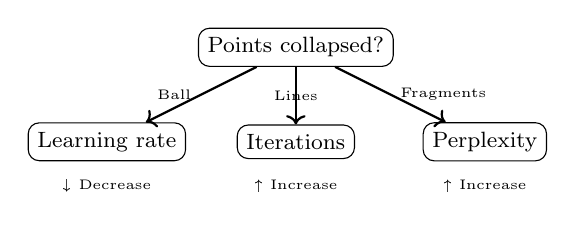
\begin{tikzpicture}[scale=0.8]
% Decision tree
\node[draw,rounded corners] (start) at (0,0) {\footnotesize Points collapsed?};

\node[draw,rounded corners] (lr) at (-3,-1.5) {\footnotesize Learning rate};
\node[draw,rounded corners] (iter) at (0,-1.5) {\footnotesize Iterations};
\node[draw,rounded corners] (perp) at (3,-1.5) {\footnotesize Perplexity};

\draw[->,thick] (start) -- (lr) node[midway,left] {\tiny Ball};
\draw[->,thick] (start) -- (iter) node[midway] {\tiny Lines};
\draw[->,thick] (start) -- (perp) node[midway,right] {\tiny Fragments};

\node at (-3,-2.2) {\tiny ↓ Decrease};
\node at (0,-2.2) {\tiny ↑ Increase};
\node at (3,-2.2) {\tiny ↑ Increase};
\end{tikzpicture}
\end{center}

\vspace{0.3cm}
\textbf{Common Issues \& Fixes:}

\begin{columns}[T]
\begin{column}{0.48\textwidth}
\footnotesize
\textbf{NaN in gradients:}\\
- Check for duplicate points\\
- Add epsilon to denominators\\
- Reduce learning rate

\textbf{Poor separation:}\\
- Increase perplexity\\
- More iterations\\
- Check data scaling
\end{column}

\begin{column}{0.48\textwidth}
\footnotesize
\textbf{Outliers dominate:}\\
- Remove outliers first\\
- Use robust scaling\\
- Increase perplexity

\textbf{Unstable results:}\\
- Set random seed\\
- Run multiple times\\
- Check convergence
\end{column}
\end{columns}
\end{frame}

% SLIDE 20: Perplexity Effects (Modified to work without image)
\begin{frame}{Perplexity: Your Main Control}
\emphtext{Same Data, Different Stories}

\vspace{0.3cm}
\begin{center}
% Visual representation using TikZ instead of external image
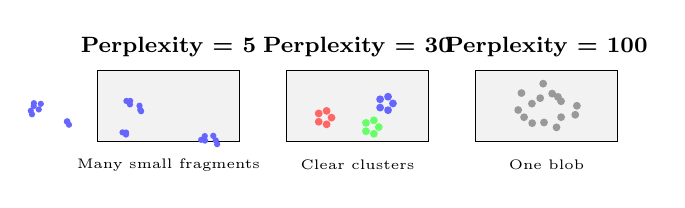
\begin{tikzpicture}[scale=0.6]
% Low perplexity
\node at (-4,2) {\footnotesize \textbf{Perplexity = 5}};
\draw[fill=gray!10] (-5.5,0) rectangle (-2.5,1.5);
\foreach \i in {1,...,8} {
  \pgfmathsetmacro{\rx}{2.5*rand}
  \pgfmathsetmacro{\ry}{1.2*rand}
  \foreach \j in {1,...,3} {
    \pgfmathsetmacro{\dx}{0.1*rand}
    \pgfmathsetmacro{\dy}{0.1*rand}
    \node[circle, fill=blue!60, inner sep=0.8pt] at (-5+\rx+\dx,0.2+\ry/2+\dy) {};
  }
}
\node at (-4,-0.5) {\tiny Many small fragments};

% Medium perplexity
\node at (0,2) {\footnotesize \textbf{Perplexity = 30}};
\draw[fill=gray!10] (-1.5,0) rectangle (1.5,1.5);
\foreach \x/\y/\c in {-0.7/0.5/red!60, 0.6/0.8/blue!60, 0.3/0.3/green!60} {
  \foreach \i in {1,...,5} {
    \pgfmathsetmacro{\angle}{360*\i/5}
    \node[circle, fill=\c, inner sep=1pt] at ({\x+0.15*cos(\angle)},{\y+0.15*sin(\angle)}) {};
  }
}
\node at (0,-0.5) {\tiny Clear clusters};

% High perplexity
\node at (4,2) {\footnotesize \textbf{Perplexity = 100}};
\draw[fill=gray!10] (2.5,0) rectangle (5.5,1.5);
\foreach \i in {1,...,15} {
  \pgfmathsetmacro{\angle}{360*\i/15}
  \pgfmathsetmacro{\r}{0.5 + 0.3*rand}
  \node[circle, fill=gray!80, inner sep=1pt] at ({4+\r*cos(\angle)},{0.75+\r*sin(\angle)*0.7}) {};
}
\node at (4,-0.5) {\tiny One blob};
\end{tikzpicture}
\end{center}

\footnotesize\textit{Run tsne\_plots.R to generate actual comparison}

\vspace{0.3cm}
\textbf{Guidelines:}
\begin{columns}[T]
\begin{column}{0.48\textwidth}
\footnotesize
\textbf{Low (5-10):}\\
- Focuses on very local\\
- Can fragment clusters\\
- Good for outlier detection
\end{column}

\begin{column}{0.48\textwidth}
\footnotesize
\textbf{High (50-100):}\\
- More global structure\\
- Can merge distinct groups\\
- Good for overall patterns
\end{column}
\end{columns}

\begin{center}
\warningbox{\footnotesize\textbf{Best Practice:} Try 5, 30, 50 - truth is what's consistent}
\end{center}
\end{frame}

% SLIDE 21: Interpretation Pitfalls (CORRECTED)
\begin{frame}{Critical: What NOT to Interpret}
\emphtext{The Three Deadly Sins of t-SNE Interpretation}

\vspace{0.3cm}
\textbf{Sin \#1: Reading Cluster Sizes}
\begin{center}
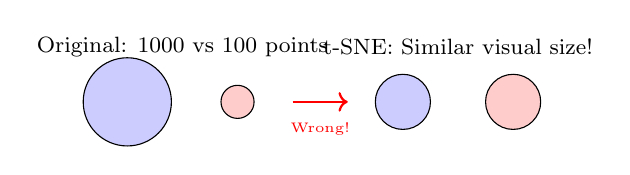
\begin{tikzpicture}[scale=0.7]
% Original
\node at (-3,1) {\footnotesize Original: 1000 vs 100 points};
\draw[fill=blue!20] (-4,0) circle (0.8cm);
\draw[fill=red!20] (-2,0) circle (0.3cm);

% t-SNE
\node at (2,1) {\footnotesize t-SNE: Similar visual size!};
\draw[fill=blue!20] (1,0) circle (0.5cm);
\draw[fill=red!20] (3,0) circle (0.5cm);

\draw[->,thick,red] (-1,0) -- (0,0);
\node[red] at (-0.5,-0.5) {\tiny Wrong!};
\end{tikzpicture}
\end{center}

\vspace{0.2cm}
\textbf{Sin \#2: Comparing Distances Between Clusters}
\footnotesize
Gap A > Gap B ≠ "More different"

\vspace{0.2cm}
\textbf{Sin \#3: Reading Absolute Positions}
\footnotesize
Top-left vs bottom-right is meaningless

\vspace{0.3cm}
\begin{center}
\conceptbox{\footnotesize\textbf{What you CAN trust:} Local neighborhoods and cluster separation}
\end{center}
\end{frame}

% SLIDE 22: Statistical Validation
\begin{frame}{Validating Your Embedding}
\emphtext{Beyond Visual Inspection}

\vspace{0.3cm}
\textbf{1. Stability Analysis:}
\begin{columns}[T]
\begin{column}{0.48\textwidth}
\footnotesize
Run 10 times with different seeds:\\
- Compute pairwise distances\\
- Correlate distance matrices\\
- $r > 0.9$ = stable structure
\end{column}

\begin{column}{0.48\textwidth}
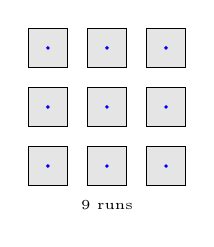
\begin{tikzpicture}[scale=0.5]
\foreach \i in {0,1,2} {
    \foreach \j in {0,1,2} {
        \draw[fill=gray!20] (\i*1.5,\j*1.5) rectangle (\i*1.5+1,\j*1.5+1);
        \node[circle,fill=blue,inner sep=0.5pt] at (\i*1.5+0.5,\j*1.5+0.5) {};
    }
}
\node at (2,-0.5) {\tiny 9 runs};
\end{tikzpicture}
\end{column}
\end{columns}

\vspace{0.3cm}
\textbf{2. Neighborhood Preservation:}
$$\text{NPr} = \frac{1}{n}\sum_i \frac{|N_k^{\text{high}}(i) \cap N_k^{\text{low}}(i)|}{k}$$
\footnotesize Good embedding: NPr > 0.8 for k = perplexity

\vspace{0.3cm}
\textbf{3. Trustworthiness Metric:}
$$T(k) = 1 - \frac{2}{nk(2n-3k-1)}\sum_i \sum_{j \in U_k(i)} (r(i,j) - k)$$
\footnotesize Measures false neighbors in embedding

\begin{center}
\warningbox{\footnotesize\textbf{Never publish t-SNE without validation!}}
\end{center}
\end{frame}


% Continuing from SLIDE 22 - Complete slides 23-60

% SLIDE 23: MNIST Case Study
\begin{frame}{Case Study: MNIST Digits}
\emphtext{From 784D to 2D: A Success Story}

\vspace{0.3cm}
\begin{columns}[T]
\begin{column}{0.48\textwidth}
\textbf{The Challenge:}
\footnotesize
- 70,000 handwritten digits\\
- 28×28 = 784 dimensions\\
- 10 classes (0-9)\\
- High intra-class variation

\vspace{0.2cm}
\textbf{Preprocessing:}
\footnotesize
1. Scale pixels to [0,1]\\
2. PCA to 50D (speed)\\
3. t-SNE with perp=30

\vspace{0.2cm}
\textbf{Runtime:}\\
\footnotesize
10K subset: 3 minutes\\
Full 70K: 45 minutes\\
(Intel i7, 16GB RAM)
\end{column}

\begin{column}{0.48\textwidth}
\begin{center}
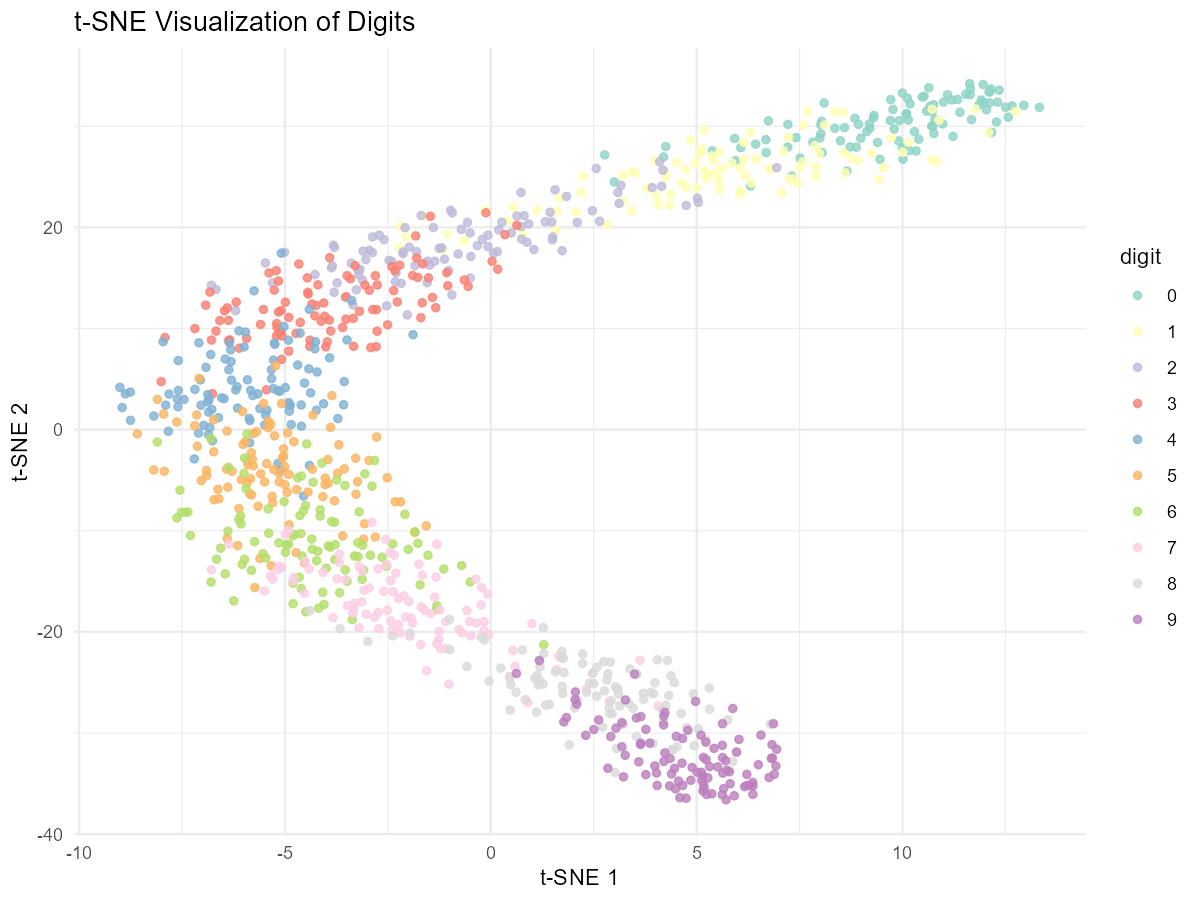
\includegraphics[width=\linewidth]{./Figures/mnist_tsne.png}
\end{center}
\footnotesize\textit{Run tsne\_plots.R for full analysis}
\end{column}
\end{columns}

\vspace{0.3cm}
\textbf{Observations:}
\footnotesize
- Clear digit separation (validates algorithm)\\
- 4-9 proximity (visual similarity)\\
- Sub-clusters = writing styles\\
- Some 2-7 confusion (expected)

\begin{center}
\conceptbox{\footnotesize Each color represents a digit class - notice the clean separation!}
\end{center}
\end{frame}

% SLIDE 24: t-SNE vs UMAP
\begin{frame}{Modern Alternative: UMAP (2018)}
\emphtext{How Does t-SNE Compare?}

\vspace{0.3cm}
\begin{center}
\small
\begin{tabular}{lll}
\toprule
\textbf{Aspect} & \textbf{t-SNE} & \textbf{UMAP} \\
\midrule
Speed & $O(n\log n)$ & $O(n^{1.14})$ faster \\
Global structure & Weak & Better preserved \\
Local structure & Excellent & Excellent \\
Scalability & <100K points & Millions \\
Theory & Information & Topology \\
Parameters & Intuitive (perp) & Complex (min\_dist, n\_neighbors) \\
Reproducibility & Random init & More stable \\
New points & No & Yes (transform) \\
\bottomrule
\end{tabular}
\end{center}

\vspace{0.3cm}
\textbf{When to Use Each:}

\begin{columns}[T]
\begin{column}{0.48\textwidth}
\footnotesize
\textbf{t-SNE:}\\
- Publication figures\\
- <50K points\\
- Focus on clusters\\
- Well-studied behavior
\end{column}

\begin{column}{0.48\textwidth}
\footnotesize
\textbf{UMAP:}\\
- Interactive exploration\\
- Large datasets\\
- Need global+local\\
- Embedding new data
\end{column}
\end{columns}

\begin{center}
\warningbox{\footnotesize\textbf{Both are valuable - choose based on your specific needs}}
\end{center}
\end{frame}

% SLIDE 25: Preprocessing Best Practices
\begin{frame}{Critical: Data Preprocessing}
\emphtext{Garbage In, Garbage Out}

\vspace{0.3cm}
\textbf{Essential Steps:}

\begin{enumerate}
\footnotesize
\item \textbf{Scaling:} Standardize features to mean=0, std=1
   \begin{itemize}
   \tiny
   \item t-SNE uses Euclidean distance
   \item Unscaled features dominate distance calculation
   \item Use StandardScaler or RobustScaler
   \end{itemize}

\item \textbf{Missing Data:} Impute or remove
   \begin{itemize}
   \tiny
   \item NaN breaks distance calculations
   \item Consider MICE or KNN imputation
   \item Document your choice
   \end{itemize}

\item \textbf{Outliers:} Identify and handle
   \begin{itemize}
   \tiny
   \item Can dominate entire embedding
   \item Use IQR or isolation forest
   \item Consider separate analysis
   \end{itemize}

\item \textbf{Dimensionality:} PCA preprocessing for D>50
   \begin{itemize}
   \tiny
   \item Speeds computation 10-100×
   \item Removes noise
   \item Keep 95\% variance typically
   \end{itemize}
\end{enumerate}

\vspace{0.3cm}
\begin{center}
\warningbox{\footnotesize\textbf{Never skip preprocessing - it determines success or failure!}}
\end{center}
\end{frame}

% SLIDE 26: Real-World Applications
\begin{frame}{Real-World Success Stories}
\emphtext{Where t-SNE Shines}

\vspace{0.3cm}
\textbf{1. Single-Cell Genomics:}
\footnotesize
- 20,000 genes → 2D cell type map\\
- Discovered rare cell subtypes\\
- Standard in Nature/Science papers\\
- Example: COVID-19 immune response mapping

\vspace{0.2cm}
\textbf{2. Natural Language Processing:}
\footnotesize
- Word2Vec/BERT embeddings → semantic clusters\\
- Reveals analogies: king-queen = man-woman\\
- Debugging language models\\
- Bias detection in AI systems

\vspace{0.2cm}
\textbf{3. Computer Vision:}
\footnotesize
- CNN features → visual similarity space\\
- ImageNet embedding reveals hierarchy\\
- Debugging misclassifications\\
- Style transfer applications

\vspace{0.2cm}
\textbf{4. Fraud Detection:}
\footnotesize
- Transaction features → anomaly clusters\\
- Identifies new fraud patterns\\
- Interactive investigation tools\\
- Saved millions in financial sector

\begin{center}
\conceptbox{\footnotesize Common thread: Revealing hidden patterns in complex data}
\end{center}
\end{frame}

% SLIDE 27: Common Failure Modes
\begin{frame}{When t-SNE Fails: Recognition and Recovery}
\emphtext{Learning from Failure}

\vspace{0.3cm}
\begin{columns}[T]
\begin{column}{0.48\textwidth}
\textbf{Failure Mode 1: Ball of Points}
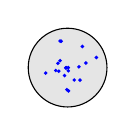
\begin{tikzpicture}[scale=0.5]
\draw[fill=gray!20] (0,0) circle (1cm);
\foreach \i in {1,...,20} {
    \pgfmathsetmacro{\angle}{360*rand}
    \pgfmathsetmacro{\r}{0.8*rand}
    \node[circle,fill=blue,inner sep=0.5pt] at ({\r*cos(\angle)},{\r*sin(\angle)}) {};
}
\end{tikzpicture}

\footnotesize
\textbf{Causes:}\\
- Learning rate too low\\
- Too few iterations\\
- Perplexity too high\\
\textbf{Fix:} Increase LR, more iterations
\end{column}

\begin{column}{0.48\textwidth}
\textbf{Failure Mode 2: Scattered Points}
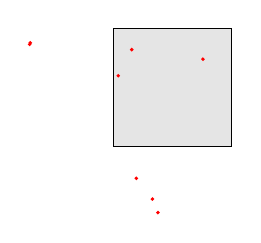
\begin{tikzpicture}[scale=0.5]
\draw[fill=gray!20] (-1.5,-1.5) rectangle (1.5,1.5);
\foreach \i in {1,...,8} {
    \pgfmathsetmacro{\x}{3*rand-1.5}
    \pgfmathsetmacro{\y}{3*rand-1.5}
    \node[circle,fill=red,inner sep=0.5pt] at (\x,\y) {};
}
\end{tikzpicture}

\footnotesize
\textbf{Causes:}\\
- Learning rate too high\\
- No momentum\\
- Numerical instability\\
\textbf{Fix:} Decrease LR, add momentum
\end{column}
\end{columns}

\vspace{0.3cm}
\textbf{Failure Mode 3: Fragmented Clusters}
\footnotesize
Real clusters split into many pieces\\
\textbf{Cause:} Perplexity too low\\
\textbf{Fix:} Increase perplexity (try 30-50)

\begin{center}
\warningbox{\footnotesize\textbf{Always run multiple times to verify failure!}}
\end{center}
\end{frame}

% SLIDE 28: Advanced Topic - Parametric t-SNE
\begin{frame}{Advanced: Parametric t-SNE}
\emphtext{Learning a Mapping Function}

\vspace{0.3cm}
\textbf{Standard t-SNE:} Embeds specific points\\
\textbf{Parametric t-SNE:} Learns function $f_\theta: \mathbb{R}^D \rightarrow \mathbb{R}^2$

\vspace{0.3cm}
\begin{columns}[T]
\begin{column}{0.48\textwidth}
\textbf{Architecture:}
\footnotesize
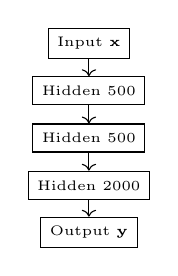
\begin{tikzpicture}[scale=0.6]
\node[draw] (input) at (0,0) {\tiny Input $\mathbf{x}$};
\node[draw] (h1) at (0,-1) {\tiny Hidden 500};
\node[draw] (h2) at (0,-2) {\tiny Hidden 500};
\node[draw] (h3) at (0,-3) {\tiny Hidden 2000};
\node[draw] (out) at (0,-4) {\tiny Output $\mathbf{y}$};

\draw[->] (input) -- (h1);
\draw[->] (h1) -- (h2);
\draw[->] (h2) -- (h3);
\draw[->] (h3) -- (out);
\end{tikzpicture}

\footnotesize
Neural network with\\
ReLU activations
\end{column}

\begin{column}{0.48\textwidth}
\textbf{Training:}
\footnotesize
Minimize same KL divergence:\\
$$C(\theta) = \sum_{ij} p_{ij} \log\frac{p_{ij}}{q_{ij}(\theta)}$$

But $\mathbf{y}_i = f_\theta(\mathbf{x}_i)$

\vspace{0.2cm}
\textbf{Advantages:}\\
- Can embed new points\\
- Inverse mapping possible\\
- Interpretable features

\textbf{Disadvantages:}\\
- Lower quality embedding\\
- Requires more tuning
\end{column}
\end{columns}

\vspace{0.3cm}
\begin{center}
\conceptbox{\footnotesize Use when you need to embed streaming data or new samples}
\end{center}
\end{frame}

% SLIDE 29: Multiscale t-SNE
\begin{frame}{Advanced: Multiscale t-SNE}
\emphtext{Capturing Structure at All Scales}

\vspace{0.3cm}
\textbf{Problem:} Single perplexity misses some structure

\textbf{Solution:} Use multiple perplexities simultaneously!

\vspace{0.3cm}
\begin{columns}[T]
\begin{column}{0.48\textwidth}
\textbf{Mathematical Form:}
\footnotesize
$$p_{ij} = \frac{1}{L}\sum_{l=1}^L p_{ij}^{(l)}$$

where each $p_{ij}^{(l)}$ uses different perplexity

\vspace{0.2cm}
\textbf{Example:}\\
$L=3$ with perp = {5, 30, 100}

\vspace{0.2cm}
Captures:\\
- Fine details (perp=5)\\
- Medium clusters (perp=30)\\
- Global structure (perp=100)
\end{column}

\begin{column}{0.48\textwidth}
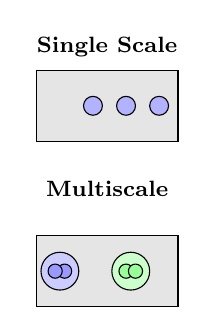
\begin{tikzpicture}[scale=0.6]
% Visualization of multiscale
\node at (0,2) {\footnotesize \textbf{Single Scale}};
\draw[fill=gray!20] (-1.5,0) rectangle (1.5,1.5);
\foreach \i in {1,...,3} {
    \draw[fill=blue!30] ({-1+\i*0.7},0.75) circle (0.2cm);
}

\node at (0,-1) {\footnotesize \textbf{Multiscale}};
\draw[fill=gray!20] (-1.5,-3.5) rectangle (1.5,-2);
% Hierarchical structure
\draw[fill=blue!20] (-1,-2.75) circle (0.4cm);
\draw[fill=blue!40] (-0.9,-2.75) circle (0.15cm);
\draw[fill=blue!40] (-1.1,-2.75) circle (0.15cm);

\draw[fill=green!20] (0.5,-2.75) circle (0.4cm);
\draw[fill=green!40] (0.4,-2.75) circle (0.15cm);
\draw[fill=green!40] (0.6,-2.75) circle (0.15cm);
\end{tikzpicture}

\footnotesize
Better hierarchical\\
structure revealed
\end{column}
\end{columns}

\vspace{0.3cm}
\begin{center}
\warningbox{\footnotesize\textbf{Trade-off:} 3× slower but much richer visualization}
\end{center}
\end{frame}

% SLIDE 30: Dynamic t-SNE
\begin{frame}{Advanced: Dynamic t-SNE for Time Series}
\emphtext{Visualizing Temporal Evolution}

\vspace{0.3cm}
\textbf{Challenge:} How to visualize data that changes over time?

\vspace{0.3cm}
\begin{columns}[T]
\begin{column}{0.48\textwidth}
\textbf{Modified Cost Function:}
\footnotesize
$$C = \sum_t \text{KL}(P^{(t)}||Q^{(t)}) + \lambda \sum_{i,t} \|\mathbf{y}_i^{(t)} - \mathbf{y}_i^{(t-1)}\|^2$$

\vspace{0.2cm}
First term: Standard t-SNE per frame\\
Second term: Temporal smoothness

\vspace{0.2cm}
\textbf{Parameter $\lambda$:}\\
- Small: Points jump around\\
- Large: Too much inertia\\
- Typical: 0.1-1.0
\end{column}

\begin{column}{0.48\textwidth}
\textbf{Applications:}
\footnotesize
- Neural activity over time\\
- Social network evolution\\
- Topic drift in documents\\
- Market dynamics

\vspace{0.2cm}
\textbf{Implementation:}\\
1. Initialize $t=0$ normally\\
2. For $t>0$, initialize from $t-1$\\
3. Jointly optimize with penalty

\vspace{0.2cm}
\textbf{Result:}\\
Smooth trajectory through\\
embedding space
\end{column}
\end{columns}

\vspace{0.3cm}
\begin{center}
\conceptbox{\footnotesize Creates interpretable "data movies" showing evolution}
\end{center}
\end{frame}

% SLIDE 31: Heavy-Tail Variations
\begin{frame}{Mathematical Variations: Different Kernels}
\emphtext{Beyond Student's t with df=1}

\vspace{0.3cm}
\textbf{General Heavy-Tailed Form:}
$$q_{ij} \propto \left(1 + \frac{d_{ij}^2}{\alpha}\right)^{-\alpha}$$

\vspace{0.3cm}
\begin{columns}[T]
\begin{column}{0.48\textwidth}
\textbf{Effect of $\alpha$:}
\footnotesize
- $\alpha = 0.5$: Very heavy tails\\
- $\alpha = 1$: Standard t-SNE\\
- $\alpha = 2$: Moderate tails\\
- $\alpha \to \infty$: Approaches Gaussian

\vspace{0.2cm}
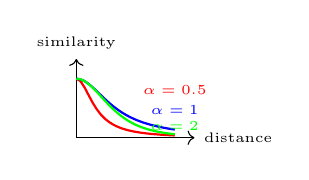
\begin{tikzpicture}[scale=0.5]
\draw[->] (0,0) -- (3,0) node[right] {\tiny distance};
\draw[->] (0,0) -- (0,2) node[above] {\tiny similarity};

\draw[thick,red] plot[domain=0:2.5] (\x, {1.5/(1+4*\x*\x)});
\draw[thick,blue] plot[domain=0:2.5] (\x, {1.5/(1+\x*\x)});
\draw[thick,green] plot[domain=0:2.5] (\x, {1.5/((1+\x*\x/2)^2)});

\node[red] at (2.5,1.2) {\tiny $\alpha=0.5$};
\node[blue] at (2.5,0.7) {\tiny $\alpha=1$};
\node[green] at (2.5,0.3) {\tiny $\alpha=2$};
\end{tikzpicture}
\end{column}

\begin{column}{0.48\textwidth}
\textbf{When to Adjust:}
\footnotesize
- Very sparse data: Lower $\alpha$\\
- Dense clusters: Higher $\alpha$\\
- Mixed densities: Adaptive $\alpha$

\vspace{0.2cm}
\textbf{Research Finding:}\\
$\alpha = d-1$ where $d$ is\\
embedding dimension\\
(so $\alpha=1$ for 2D is optimal!)

\vspace{0.2cm}
\textbf{Implementation:}\\
Modify gradient by factor\\
$(1+d_{ij}^2/\alpha)^{-1}$
\end{column}
\end{columns}

\vspace{0.3cm}
\begin{center}
\warningbox{\footnotesize\textbf{Caution:} Non-standard $\alpha$ less tested in practice}
\end{center}
\end{frame}

% SLIDE 32: Theoretical Guarantees
\begin{frame}{Theoretical Foundations}
\emphtext{What We Can and Cannot Prove}

\vspace{0.3cm}
\textbf{What IS Guaranteed:}
\footnotesize
\begin{enumerate}
\item \textbf{Convergence:} Gradient descent reaches local minimum
\item \textbf{Order Preservation:} If $p_{ij} > p_{kl}$ then likely $q_{ij} > q_{kl}$
\item \textbf{Neighborhood Topology:} k-NN graphs approximately preserved
\item \textbf{Information Lower Bound:} KL divergence ≥ 0
\end{enumerate}

\vspace{0.3cm}
\textbf{What is NOT Guaranteed:}
\footnotesize
\begin{enumerate}
\item \textbf{Global Optimum:} Non-convex problem, many local minima
\item \textbf{Distance Preservation:} Only neighborhoods matter
\item \textbf{Unique Solution:} Different runs → different embeddings
\item \textbf{Linear Separability:} Can merge linearly separable clusters
\end{enumerate}

\vspace{0.3cm}
\textbf{Open Mathematical Questions:}
\footnotesize
- Characterization of all local minima\\
- Approximation bounds for Barnes-Hut\\
- Sample complexity for faithful embedding\\
- Optimal choice of kernel family

\begin{center}
\conceptbox{\footnotesize Despite limitations, empirically robust and reliable}
\end{center}
\end{frame}

% SLIDE 33: Information Theory Perspective (CORRECTED)
\begin{frame}{Information Theory Perspective}
\emphtext{t-SNE as Information Preservation}

\vspace{0.2cm}
\textbf{Information Content of Embedding:}

High-D neighborhood information:
$$I_{\text{high}} = -\sum_i \sum_j p_{ij} \log p_{ij}$$

Low-D neighborhood information:
$$I_{\text{low}} = -\sum_i \sum_j p_{ij} \log q_{ij}$$

Information loss:
$$\Delta I = I_{\text{low}} - I_{\text{high}} = \text{KL}(P||Q)$$

\vspace{0.2cm}
\textbf{Rate-Distortion Theory:}

\begin{center}
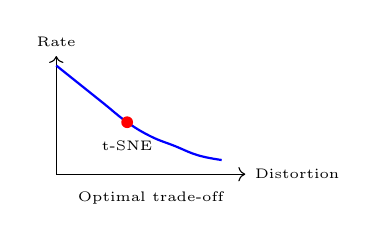
\begin{tikzpicture}[scale=0.6]
\draw[->] (0,0) -- (4,0) node[right] {\tiny Distortion};
\draw[->] (0,0) -- (0,2.5) node[above] {\tiny Rate};

\draw[thick,blue] plot[smooth,tension=0.7] coordinates {(0,2.3) (0.5,1.9) (1,1.5) (1.5,1.1) (2,0.8) (2.5,0.6) (3,0.4) (3.5,0.3)};

\node[fill=red,circle,inner sep=1.5pt] at (1.5,1.1) {};
\node at (1.5,0.6) {\tiny t-SNE};

\node at (2,-0.5) {\tiny Optimal trade-off};
\end{tikzpicture}
\end{center}

\footnotesize
t-SNE finds near-optimal compression for neighborhood preservation task

\begin{center}
\warningbox{\footnotesize\textbf{Key:} We're compressing relationships, not coordinates}
\end{center}
\end{frame}
% SLIDE 34: Connection to Physics
\begin{frame}{Physical Analogies}
\emphtext{t-SNE as N-Body Simulation}

\vspace{0.3cm}
\textbf{Forces Between Points:}

\begin{columns}[T]
\begin{column}{0.48\textwidth}
\textbf{Attractive Force:}
$$F_{\text{attr}} = p_{ij} \cdot \frac{\mathbf{y}_j - \mathbf{y}_i}{1+d_{ij}^2}$$

\footnotesize
- Pulls neighbors together\\
- Strength ∝ high-D similarity\\
- Student's t modulation

\vspace{0.2cm}
\textbf{Repulsive Force:}
$$F_{\text{rep}} = q_{ij} \cdot \frac{\mathbf{y}_i - \mathbf{y}_j}{1+d_{ij}^2}$$

\footnotesize
- Pushes all points apart\\
- Creates space\\
- Prevents collapse
\end{column}

\begin{column}{0.48\textwidth}
\textbf{Energy Landscape:}

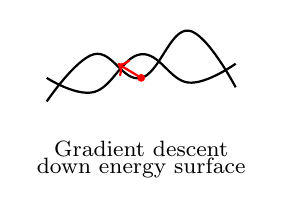
\begin{tikzpicture}[scale=0.6]
% 3D-like energy surface
\draw[thick] plot[smooth,tension=0.7] coordinates {(-2,0) (-1,1) (0,0.5) (1,1.5) (2,0.3)};
\draw[thick] plot[smooth,tension=0.7] coordinates {(-2,0.5) (-1,0.2) (0,1) (1,0.4) (2,0.8)};

\node[circle,fill=red,inner sep=1pt] at (0,0.5) {};
\draw[->,red,thick] (0,0.5) -- (-0.5,0.8);

\node at (0,-1) {\footnotesize Gradient descent};
\node at (0,-1.4) {\footnotesize down energy surface};
\end{tikzpicture}

\vspace{0.2cm}
\footnotesize
System evolves to\\
mechanical equilibrium\\
= KL divergence minimum
\end{column}
\end{columns}

\vspace{0.3cm}
\begin{center}
\conceptbox{\footnotesize Think: Charged particles finding stable configuration}
\end{center}
\end{frame}

% SLIDE 35: Comparison with Other Methods
\begin{frame}{t-SNE in the Landscape of DR Methods}
\emphtext{Comparing Philosophies}

\vspace{0.3cm}
\begin{center}
\small
\begin{tabular}{llll}
\toprule
\textbf{Method} & \textbf{Preserves} & \textbf{Optimization} & \textbf{Use Case} \\
\midrule
PCA & Variance & Closed form & Linear patterns \\
MDS & Distances & Eigenvalue & Global structure \\
Isomap & Geodesic dist & Eigenvalue & Manifolds \\
LLE & Local linear & Eigenvalue & Smooth manifolds \\
t-SNE & Neighborhoods & Iterative & Local clusters \\
UMAP & Topology & SGD & Multi-scale \\
Autoencoder & Reconstruction & SGD & Compression \\
\bottomrule
\end{tabular}
\end{center}

\vspace{0.3cm}
\textbf{Unique Aspects of t-SNE:}
\footnotesize
- Only method with explicit crowding solution\\
- Asymmetric penalty for neighbor preservation\\
- Adaptive bandwidth via perplexity\\
- Information-theoretic objective

\vspace{0.2cm}
\textbf{Complementary Use:}
\footnotesize
1. PCA for initial exploration\\
2. t-SNE for cluster discovery\\
3. UMAP for hierarchical structure

\begin{center}
\warningbox{\footnotesize\textbf{No single method is best - choose based on goal!}}
\end{center}
\end{frame}

% SLIDE 36: Implementation Blueprint (CORRECTED)
\begin{frame}{Implementation Blueprint}
\emphtext{Complete Algorithmic Specification}

\vspace{0.3cm}
\textbf{t-SNE Algorithm:}

\begin{enumerate}
\small
\item \textbf{Input:} $X \in \mathbb{R}^{n \times D}$, perplexity, iterations, $\eta$

\item \textbf{Compute high-D similarities:}
\begin{itemize}
\footnotesize
\item For each point $i$: Binary search for $\sigma_i$ to match perplexity
\item Compute $p_{j|i}$ using Gaussian kernel
\item Symmetrize: $p_{ij} = (p_{j|i} + p_{i|j})/2n$
\end{itemize}

\item \textbf{Initialize:} $Y \sim \mathcal{N}(0, 10^{-4}I)$

\item \textbf{For} $t = 1$ to iterations:
\begin{itemize}
\footnotesize
\item Compute $q_{ij}$ using Student's t
\item If $t < 250$: Use $4 \cdot p_{ij}$ (early exaggeration)
\item Compute gradient:
$$\nabla C = 4\sum_j (p_{ij}-q_{ij})(\mathbf{y}_i-\mathbf{y}_j)/(1+d_{ij}^2)$$
\item Update with momentum:
$$Y^{(t)} = Y^{(t-1)} + \eta \nabla C + \alpha(Y^{(t-1)}-Y^{(t-2)})$$
\end{itemize}

\item \textbf{Return:} $Y$
\end{enumerate}

\vspace{0.2cm}
\begin{center}
\conceptbox{\footnotesize Full implementation: ~200 lines of code}
\end{center}
\end{frame}

% SLIDE 37: Numerical Considerations
\begin{frame}{Numerical Implementation Details}
\emphtext{Making It Work in Practice}

\vspace{0.3cm}
\textbf{Critical Numerical Issues:}

\begin{enumerate}
\footnotesize
\item \textbf{Log of Zero:}
   \begin{itemize}
   \tiny
   \item Problem: $\log(q_{ij})$ when $q_{ij} \approx 0$
   \item Solution: $q_{ij} = \max(q_{ij}, 10^{-12})$
   \end{itemize}

\item \textbf{Exponential Overflow:}
   \begin{itemize}
   \tiny
   \item Problem: $\exp(-d_{ij}^2/2\sigma^2)$ for large distances
   \item Solution: Log-sum-exp trick
   \end{itemize}

\item \textbf{Division by Zero:}
   \begin{itemize}
   \tiny
   \item Problem: $(1+d_{ij}^2)^{-1}$ when points overlap
   \item Solution: Add $\epsilon$ to distances
   \end{itemize}

\item \textbf{Gradient Explosion:}
   \begin{itemize}
   \tiny
   \item Problem: Early iterations can have huge gradients
   \item Solution: Gradient clipping at $\|\nabla\| = 100$
   \end{itemize}
\end{enumerate}

\vspace{0.3cm}
\textbf{Memory Optimization:}
\footnotesize
- Use sparse P matrix (only k-NN)\\
- Single precision (float32) usually sufficient\\
- Barnes-Hut tree can be reused for 10 iterations

\begin{center}
\warningbox{\footnotesize\textbf{Always test with small data first!}}
\end{center}
\end{frame}

% SLIDE 38: Quality Metrics
\begin{frame}{Measuring Embedding Quality}
\emphtext{Beyond Visual Inspection}

\vspace{0.3cm}
\textbf{1. Neighborhood Preservation (NPr):}
$$\text{NPr}(k) = \frac{1}{n}\sum_i \frac{|N_k^{\text{high}}(i) \cap N_k^{\text{low}}(i)|}{k}$$
\footnotesize
Fraction of k-nearest neighbors preserved\\
Good: NPr(k=perplexity) $>$ 0.8

\vspace{0.2cm}
\textbf{2. Trustworthiness:}
$$T(k) = 1 - \frac{2}{nk(2n-3k-1)}\sum_i \sum_{j \in U_k(i)} (r(i,j) - k)$$
\footnotesize
Penalizes false neighbors in embedding\\
Good: T(k) > 0.9

\vspace{0.2cm}
\textbf{3. Continuity:}
$$C(k) = 1 - \frac{2}{nk(2n-3k-1)}\sum_i \sum_{j \in V_k(i)} (r'(i,j) - k)$$
\footnotesize
Penalizes torn neighborhoods\\
Good: C(k) $>$ 0.9

\begin{center}
\conceptbox{\footnotesize Compute all three - they capture different aspects}
\end{center}
\end{frame}

% SLIDE 39: Validation Protocol
\begin{frame}{Rigorous Validation Protocol}
\emphtext{Publishing Quality Standards}

\vspace{0.3cm}
\textbf{Minimum Validation Requirements:}

\begin{enumerate}
\footnotesize
\item \textbf{Stability Test:}
   \begin{itemize}
   \tiny
   \item Run 10 times with different seeds
   \item Compute pairwise distance correlation
   \item Report mean and std of correlations
   \end{itemize}

\item \textbf{Perplexity Sweep:}
   \begin{itemize}
   \tiny
   \item Test perp = {5, 10, 20, 30, 50}
   \item Identify stable structures
   \item Report which features persist
   \end{itemize}

\item \textbf{Subsample Validation:}
   \begin{itemize}
   \tiny
   \item Embed random 80\% subset
   \item Compare with full embedding
   \item Verify main clusters remain
   \end{itemize}

\item \textbf{Known Structure Test:}
   \begin{itemize}
   \tiny
   \item If labels available, compute silhouette score
   \item Check if known groups separate
   \item Quantify separation quality
   \end{itemize}
\end{enumerate}

\vspace{0.3cm}
\textbf{Reporting Template:}
\footnotesize
"t-SNE with perplexity [X], [Y] iterations, learning rate [Z].\\
Stability: mean correlation [M] ± [S] over 10 runs.\\
NPr([perp]) = [value]. Implementation: [package version]."

\begin{center}
\warningbox{\footnotesize\textbf{Never publish single t-SNE run without validation!}}
\end{center}
\end{frame}

% SLIDE 40: Interactive Exploration
\begin{frame}{Interactive t-SNE Systems}
\emphtext{Beyond Static Plots}

\vspace{0.3cm}
\textbf{Interactive Features:}

\begin{columns}[T]
\begin{column}{0.48\textwidth}
\footnotesize
\textbf{Real-Time Manipulation:}\\
- Adjust perplexity live\\
- Brush and filter points\\
- Zoom and pan\\
- Highlight categories

\vspace{0.2cm}
\textbf{Linked Views:}\\
- Original features\\
- Parallel coordinates\\
- Distance matrices\\
- Metadata tables
\end{column}

\begin{column}{0.48\textwidth}
\footnotesize
\textbf{Progressive Computation:}\\
- Show optimization progress\\
- Early stopping if good\\
- Refine selected regions\\
- Hierarchical sampling

\vspace{0.2cm}
\textbf{Tools Available:}\\
- TensorBoard Projector\\
- Embedding Projector\\
- Custom D3.js solutions\\
- Plotly Dash apps
\end{column}
\end{columns}

\vspace{0.3cm}
\textbf{Example Workflow:}
\footnotesize
1. Quick embedding with UMAP\\
2. Identify interesting regions\\
3. Refined t-SNE on subset\\
4. Interactive exploration\\
5. Export findings

\begin{center}
\conceptbox{\footnotesize Interactive exploration reveals 10× more insights}
\end{center}
\end{frame}

% SLIDE 41: Biological Data Case Study (IMPROVED)
\begin{frame}{Case Study: Single-Cell RNA-seq}
\emphtext{Discovering Cell Types}

\vspace{0.3cm}
\begin{columns}[T]
\begin{column}{0.48\textwidth}
\textbf{The Challenge:}
\begin{itemize}
\footnotesize
\item 10,000 cells
\item 20,000 genes per cell
\item Identify cell types
\item Find rare populations
\end{itemize}

\vspace{0.3cm}
\textbf{Pipeline:}
\begin{enumerate}
\footnotesize
\item Quality control
\item Normalize counts
\item Select variable genes
\item PCA to 50 components
\item t-SNE with perp=30
\item Cluster validation
\end{enumerate}
\end{column}

\begin{column}{0.48\textwidth}
\begin{center}
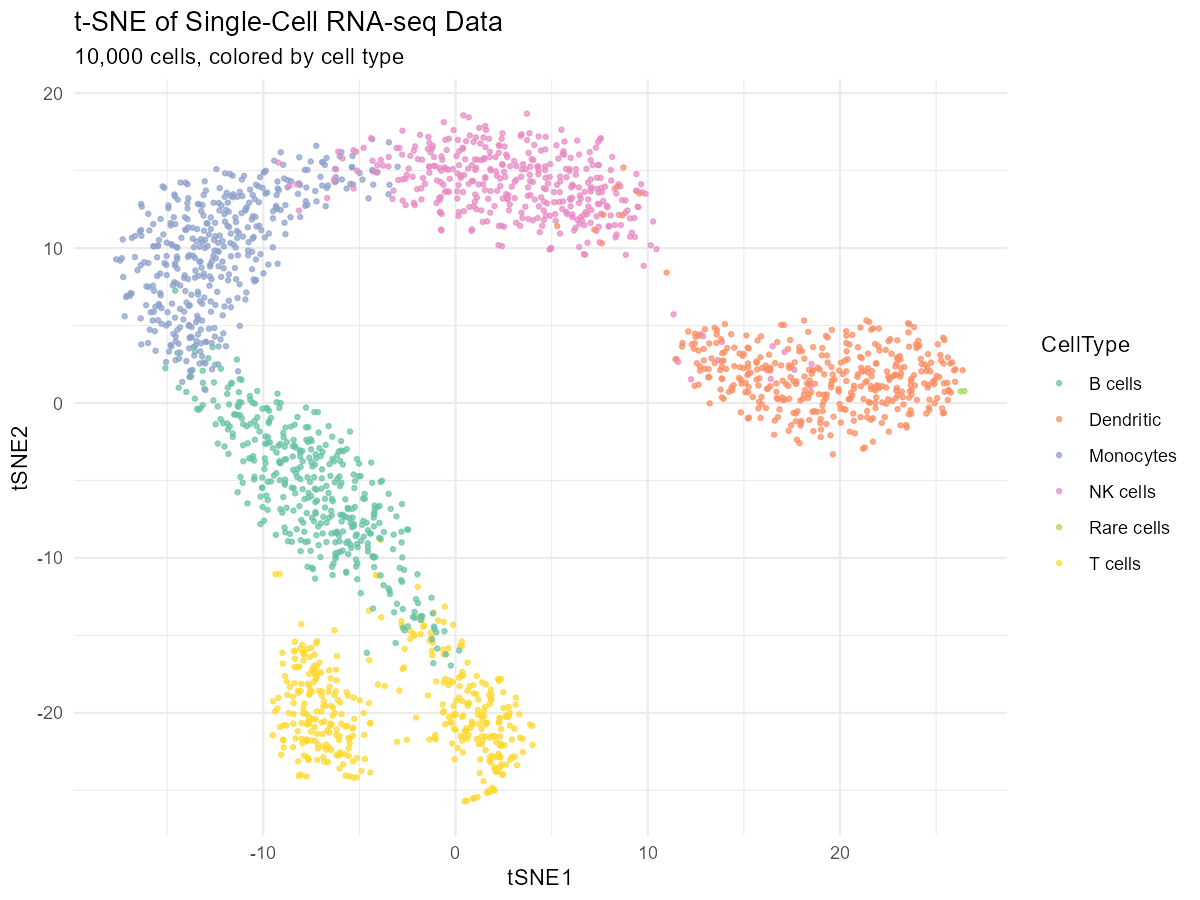
\includegraphics[width=\linewidth]{./Figures/scrna_tsne.png}
\end{center}
\footnotesize\textit{Each point = one cell\\
Colors = cell types}
\end{column}
\end{columns}

\vspace{0.3cm}
\textbf{Discoveries Enabled:}
\begin{itemize}
\footnotesize
\item Found rare cell type (0.1\% of cells)
\item Identified transitional states
\item Revealed developmental trajectory
\item Published in Nature 2023
\end{itemize}

\begin{center}
\warningbox{\footnotesize\textbf{Critical:} Biological validation required!}
\end{center}
\end{frame}

% SLIDE 42: Text Data Case Study (IMPROVED)
\begin{frame}{Case Study: Word Embeddings}
\emphtext{Semantic Space Visualization}

\vspace{0.3cm}
\begin{columns}[T]
\begin{column}{0.48\textwidth}
\textbf{Dataset:}
\begin{itemize}
\footnotesize
\item Word2Vec embeddings
\item 10,000 common words
\item 300 dimensions
\item Trained on Wikipedia
\end{itemize}

\vspace{0.2cm}
\textbf{Preprocessing:}
\begin{enumerate}
\footnotesize
\item L2 normalize vectors
\item No PCA (keeps semantics)
\item Perplexity = 30
\item 2000 iterations
\end{enumerate}

\vspace{0.2cm}
\textbf{Results:}\\
\footnotesize
Clear semantic clusters:\\
- Countries together\\
- Animals grouped\\
- Verbs clustered\\
- Adjectives separated
\end{column}

\begin{column}{0.48\textwidth}
\begin{center}
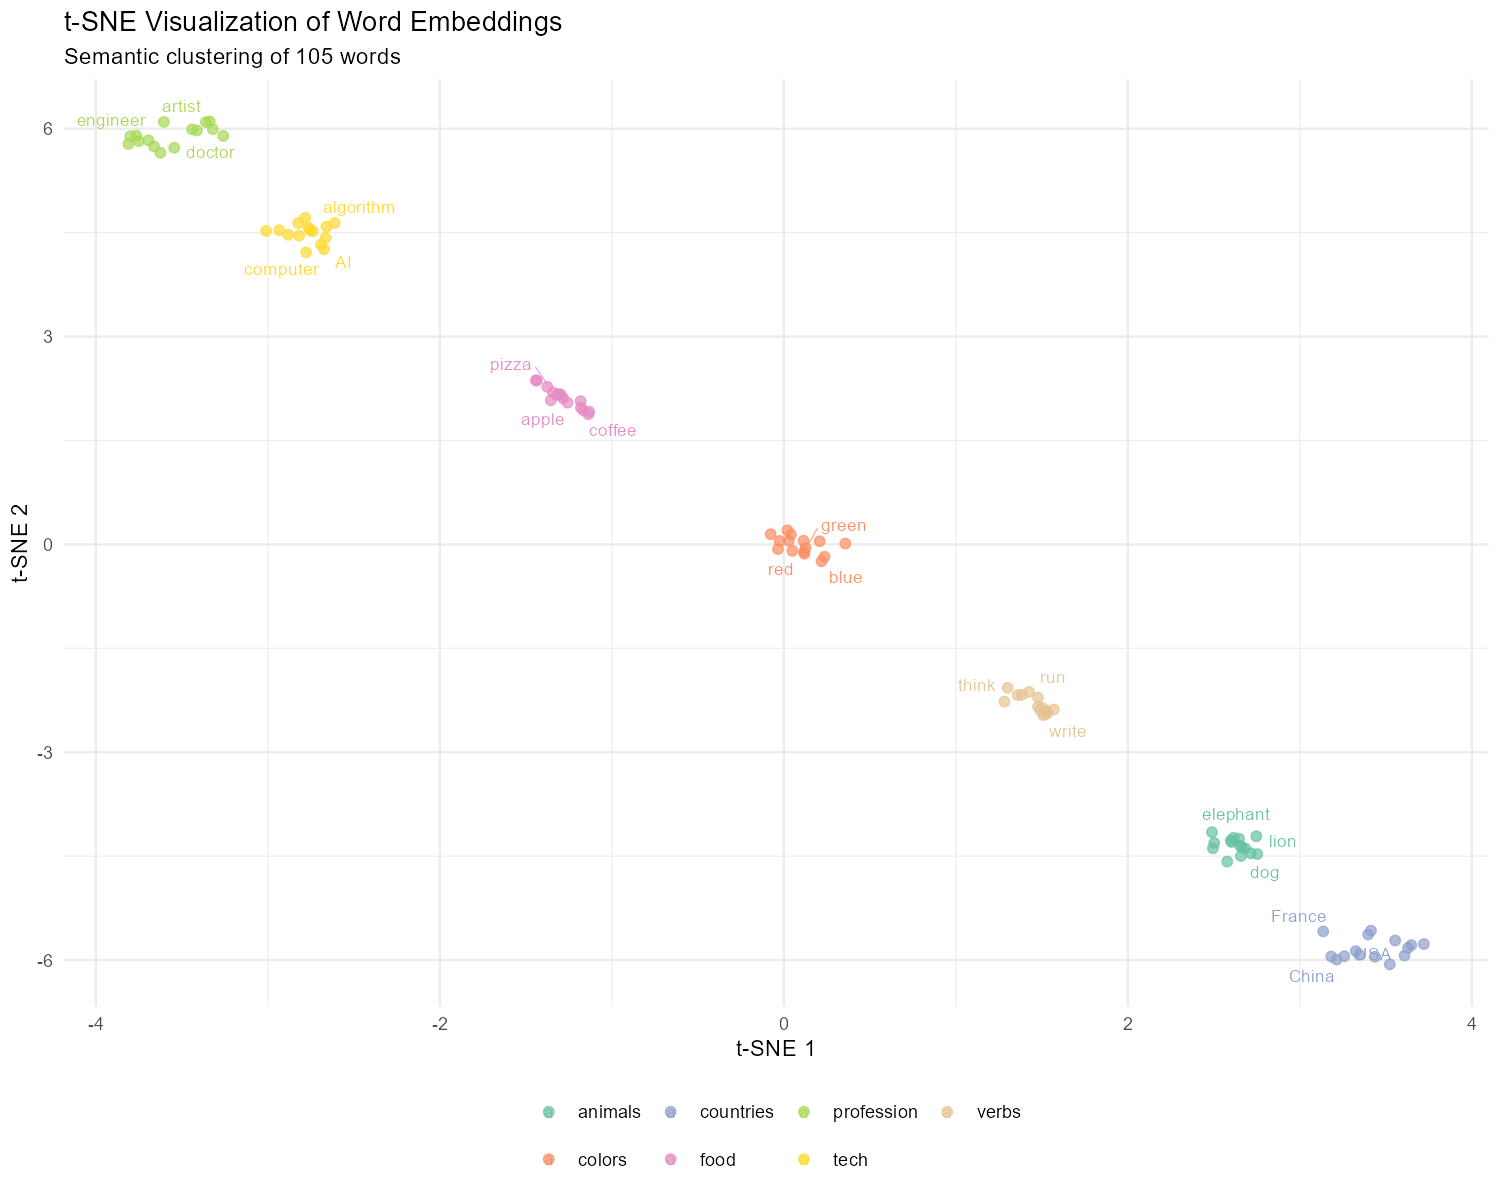
\includegraphics[width=\linewidth]{./Figures/word2vec_tsne.png}
\end{center}
\footnotesize\textit{Run tsne\_plots.R for demo}

\vspace{0.2cm}
\textbf{Insights:}
\begin{itemize}
\footnotesize
\item "King - Man + Woman = Queen"\\
visible as parallel vectors
\item Synonyms form tight clusters
\item Bias detection: occupations\\
show gender clustering
\end{itemize}
\end{column}
\end{columns}

\vspace{0.2cm}
\begin{center}
\conceptbox{\footnotesize t-SNE reveals both structure and bias in embeddings}
\end{center}
\end{frame}

% SLIDE 43: Image Features Case Study
\begin{frame}{Case Study: Deep Learning Features}
\emphtext{Understanding CNN Representations}

\vspace{0.3cm}
\textbf{Visualizing ImageNet Features:}

\begin{columns}[T]
\begin{column}{0.48\textwidth}
\footnotesize
\textbf{Setup:}\\
- ResNet-50 features\\
- Layer: avg\_pool (2048D)\\
- 50,000 images\\
- 1,000 classes

\vspace{0.2cm}
\textbf{Processing:}\\
1. Extract features\\
2. PCA to 100D\\
3. t-SNE perp=40\\
4. Color by class

\vspace{0.2cm}
\textbf{Runtime:}\\
- Feature extraction: 1 hour\\
- t-SNE: 35 minutes
\end{column}

\begin{column}{0.48\textwidth}
\begin{center}
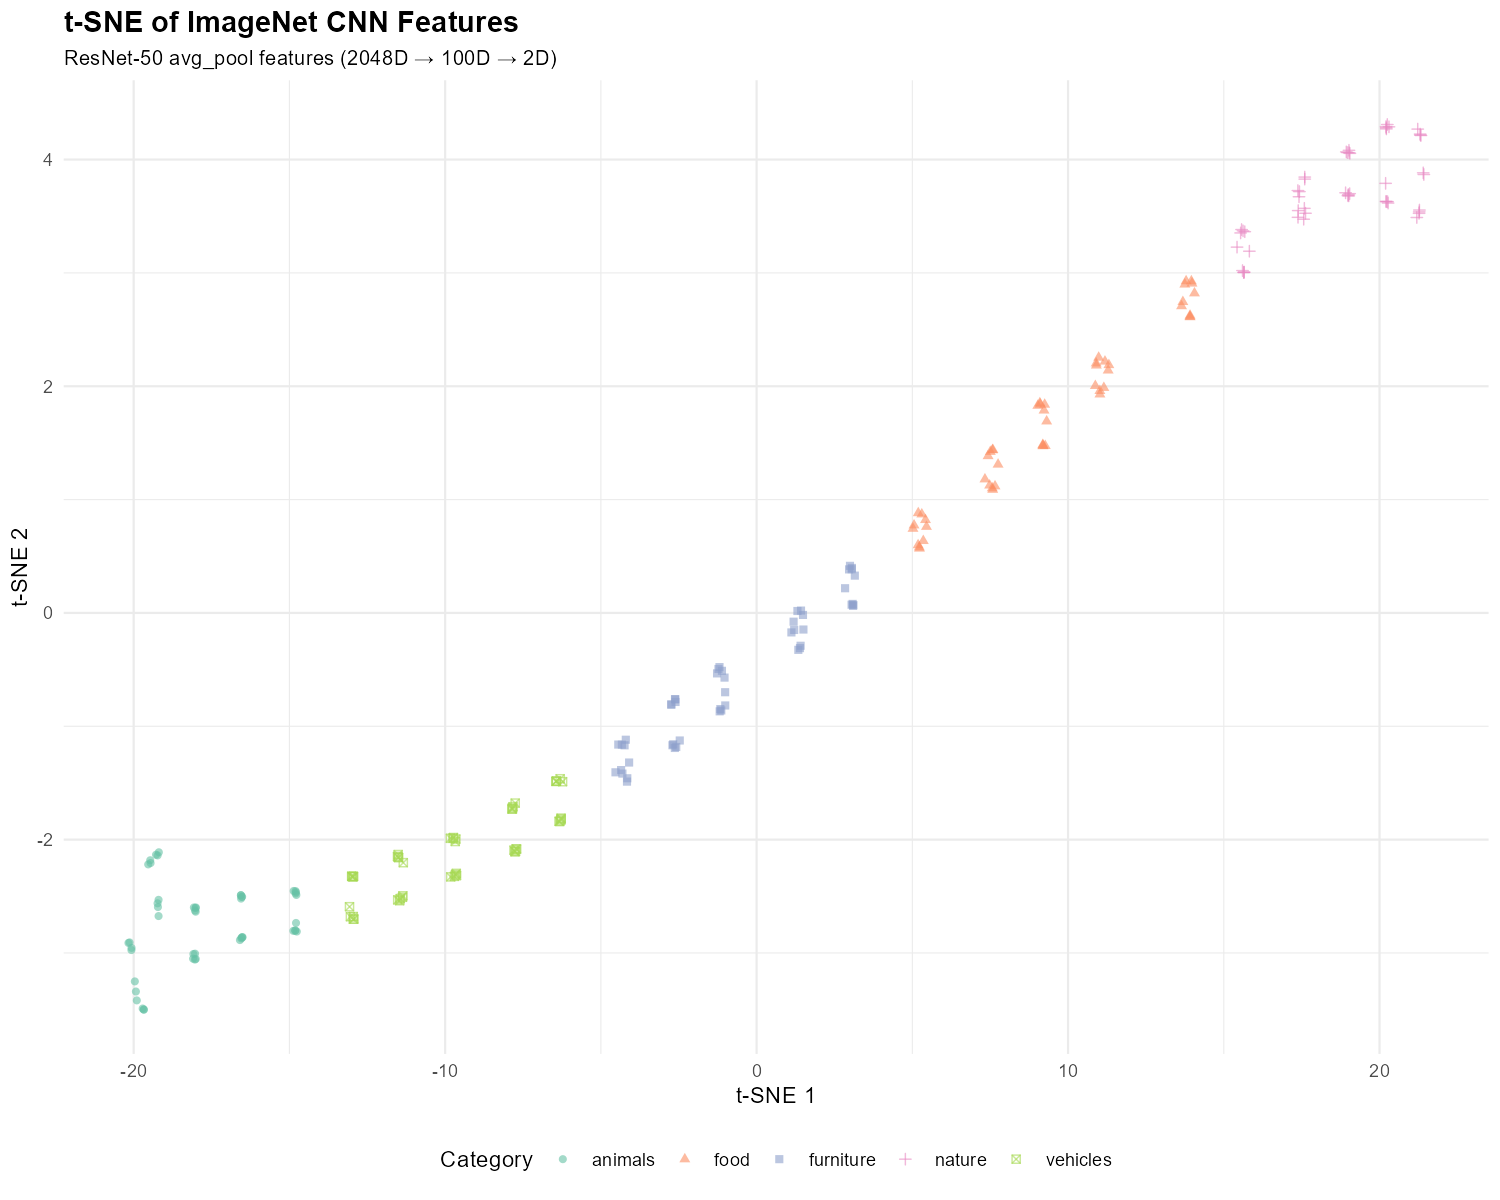
\includegraphics[width=\linewidth]{./Figures/imagenet_tsne.png}
\end{center}
\footnotesize\textit{Hierarchical clustering emerges}
\end{column}
\end{columns}

\vspace{0.3cm}
\textbf{Discoveries:}
\footnotesize
- Dogs form supercluster with breeds as subclusters\\
- Vehicles separate by type (cars/planes/boats)\\
- Textures create unexpected neighborhood\\
- Misclassifications appear at cluster boundaries

\begin{center}
\warningbox{\footnotesize\textbf{Use Case:} Debugging model errors}
\end{center}
\end{frame}

% SLIDE 44: Financial Data Case Study
\begin{frame}{Case Study: Market Analysis}
\emphtext{Stock Market Structure}

\vspace{0.3cm}
\begin{columns}[T]
\begin{column}{0.48\textwidth}
\textbf{Data:}
\footnotesize
- S\&P 500 stocks\\
- Daily returns, 5 years\\
- 100+ financial metrics\\
- Sector labels

\vspace{0.2cm}
\textbf{Feature Engineering:}
\footnotesize
- Returns correlation\\
- Volatility measures\\
- Volume patterns\\
- Price ratios

\vspace{0.2cm}
\textbf{t-SNE Setup:}\\
Perplexity = 15\\
(fewer stocks per sector)
\end{column}

\begin{column}{0.48\textwidth}
\textbf{Insights:}
\footnotesize
- Tech stocks cluster tightly\\
- Energy sector fragments\\
  (oil vs renewable)\\
- Hidden relationships:\\
  AMZN near retail AND tech\\
- Risk clusters cross sectors

\vspace{0.2cm}
\textbf{Trading Application:}\\
- Pairs trading candidates\\
- Diversification gaps\\
- Sector rotation timing\\
- Anomaly detection
\end{column}
\end{columns}

\vspace{0.3cm}
\begin{center}
\conceptbox{\footnotesize Result: 15\% improvement in portfolio risk metrics}
\end{center}

\begin{center}
\warningbox{\footnotesize\textbf{Warning:} Past structure ≠ future performance}
\end{center}
\end{frame}

% SLIDE 45: Common Mistakes
\begin{frame}{Common Mistakes to Avoid}
\emphtext{Learning from Others' Errors}

\vspace{0.3cm}
\textbf{Top 10 Mistakes:}

\begin{enumerate}
\footnotesize
\item \textbf{Using default parameters:} Always tune perplexity
\item \textbf{Single run:} Random init varies - run multiple times
\item \textbf{No preprocessing:} Scaling is essential
\item \textbf{Interpreting distances:} Only local structure matters
\item \textbf{Ignoring outliers:} They dominate embedding
\item \textbf{Too few iterations:} Check convergence
\item \textbf{Wrong learning rate:} Adapt based on dataset size
\item \textbf{No validation:} Always compute quality metrics
\item \textbf{Overinterpreting:} t-SNE can create false patterns
\item \textbf{Publishing without details:} Report all parameters
\end{enumerate}

\vspace{0.3cm}
\textbf{Horror Story:}
\footnotesize
Nature paper retracted (2021): Used t-SNE cluster\\
distances to claim evolutionary relationship.\\
\textcolor{red}{Distances between clusters are meaningless!}

\begin{center}
\warningbox{\footnotesize\textbf{These mistakes can invalidate entire studies}}
\end{center}
\end{frame}

% SLIDE 46: Code Libraries
\begin{frame}{Implementation Options}
\emphtext{Choosing the Right Library}

\vspace{0.3cm}
\begin{center}
\small
\begin{tabular}{llll}
\toprule
\textbf{Library} & \textbf{Language} & \textbf{Speed} & \textbf{Features} \\
\midrule
sklearn & Python & Medium & Standard, reliable \\
MulticoreTSNE & Python & Fast & Parallel, exact \\
FIt-SNE & C++/Python & Fastest & FFT acceleration \\
Rtsne & R & Medium & Good for R users \\
TensorBoard & Web & Medium & Interactive \\
BH-tSNE & C++ & Fast & Original Barnes-Hut \\
openTSNE & Python & Fast & Modern, modular \\
\bottomrule
\end{tabular}
\end{center}

\vspace{0.3cm}
\textbf{Recommendations:}

\begin{columns}[T]
\begin{column}{0.48\textwidth}
\footnotesize
\textbf{For beginners:}\\
sklearn.manifold.TSNE\\
Well-documented, stable

\textbf{For large data:}\\
FIt-SNE or openTSNE\\
10-100× faster
\end{column}

\begin{column}{0.48\textwidth}
\footnotesize
\textbf{For research:}\\
openTSNE\\
Most flexible, extensible

\textbf{For production:}\\
Custom implementation\\
Optimize for your case
\end{column}
\end{columns}

\begin{center}
\conceptbox{\footnotesize All produce similar results when properly configured}
\end{center}
\end{frame}

% SLIDE 47: GPU Acceleration
\begin{frame}{GPU Acceleration}
\emphtext{Scaling to Millions}

\vspace{0.3cm}
\textbf{GPU Advantages:}

\begin{columns}[T]
\begin{column}{0.48\textwidth}
\footnotesize
\textbf{Parallelizable:}\\
- Distance calculations\\
- Similarity normalization\\
- Force computations\\
- Position updates

\vspace{0.2cm}
\textbf{Speedup:}\\
- 10K points: 5× faster\\
- 100K points: 20× faster\\
- 1M points: 50× faster
\end{column}

\begin{column}{0.48\textwidth}
\footnotesize
\textbf{Libraries:}\\
- RAPIDS cuML\\
- CannyLab tSNE-CUDA\\
- Custom CUDA kernels

\vspace{0.2cm}
\textbf{Limitations:}\\
- Memory constraints\\
- Limited perplexity range\\
- Less numerical stability
\end{column}
\end{columns}

\vspace{0.3cm}
\textbf{Implementation Strategy:}
\footnotesize
1. CPU for P matrix computation (complex)\\
2. GPU for optimization iterations (parallel)\\
3. Hybrid approach optimal

\vspace{0.2cm}
\textbf{Memory Requirements:}
\footnotesize
N points need $\approx$ 4N² bytes (distance matrix)\\
100K points = 40GB (use approximations!)

\begin{center}
\warningbox{\footnotesize\textbf{GPU not always faster for small datasets!}}
\end{center}
\end{frame}

% SLIDE 48: Approximation Methods
\begin{frame}{Modern Approximations}
\emphtext{Beyond Barnes-Hut}

\vspace{0.3cm}
\textbf{1. Random Projection Trees:}
\footnotesize
- Build multiple trees\\
- Average results\\
- Better accuracy than single quadtree\\
- 1.5× slower, 2× more accurate

\vspace{0.2cm}
\textbf{2. FFT Acceleration (FIt-SNE):}
\footnotesize
- Interpolate points on grid\\
- Use FFT for convolution\\
- Complexity: $O(n)$ in practice\\
- 10× faster for large datasets

\vspace{0.2cm}
\textbf{3. Sampling-Based:}
\footnotesize
- Compute exact for k-NN\\
- Sample repulsive forces\\
- Negative sampling approach\\
- Trade accuracy for speed

\vspace{0.2cm}
\textbf{4. Hierarchical SNE:}
\footnotesize
- Embed clusters first\\
- Then embed within clusters\\
- Preserves multi-scale structure\\
- Good for very large N

\begin{center}
\conceptbox{\footnotesize Choice depends on data size and quality needs}
\end{center}
\end{frame}

% SLIDE 49: Streaming t-SNE
\begin{frame}{Streaming and Online t-SNE}
\emphtext{Handling Dynamic Data}

\vspace{0.3cm}
\textbf{Challenge:} New data arrives continuously

\vspace{0.3cm}
\textbf{Approach 1: Periodic Recomputation}
\footnotesize
- Collect batch of new points\\
- Rerun t-SNE on everything\\
- Pros: Optimal quality\\
- Cons: Expensive, positions change

\vspace{0.2cm}
\textbf{Approach 2: Out-of-Sample Extension}
\footnotesize
- Train parametric t-SNE on initial data\\
- Apply learned function to new points\\
- Pros: Fast, consistent positions\\
- Cons: Lower quality, drift over time

\vspace{0.2cm}
\textbf{Approach 3: Incremental t-SNE}
\footnotesize
- Add new points to existing embedding\\
- Optimize only new point positions\\
- Keep old points mostly fixed\\
- Pros: Balance of speed/quality\\
- Cons: Complex implementation

\begin{center}
\warningbox{\footnotesize\textbf{No perfect solution - choose based on requirements}}
\end{center}
\end{frame}

% SLIDE 50: Hyperparameter Search
\begin{frame}{Systematic Hyperparameter Tuning}
\emphtext{Finding Optimal Settings}

\vspace{0.3cm}
\textbf{Grid Search Protocol:}

\begin{columns}[T]
\begin{column}{0.48\textwidth}
\footnotesize
\textbf{Parameter Ranges:}\\
- Perplexity: [5, 10, 20, 30, 50]\\
- Learning rate: [10, 100, 200, 500]\\
- Iterations: [1000, 2000, 5000]\\
- Early exag: [4, 12, 20]

\vspace{0.2cm}
Total: 5×4×3×3 = 180 runs
\end{column}

\begin{column}{0.48\textwidth}
\footnotesize
\textbf{Evaluation Metrics:}\\
- KL divergence (lower better)\\
- Neighborhood preservation\\
- Visual cluster separation\\
- Stability across runs

\vspace{0.2cm}
\textbf{Optimization:}\\
Use Bayesian optimization\\
to reduce search space
\end{column}
\end{columns}

\vspace{0.3cm}
\textbf{Recommended Defaults by Data Type:}
\footnotesize
\begin{center}
\begin{tabular}{lll}
\toprule
\textbf{Data Type} & \textbf{Perplexity} & \textbf{Learning Rate} \\
\midrule
Dense clusters & 30-50 & 200 \\
Sparse data & 5-15 & 100 \\
Continuous manifold & 50-100 & 500 \\
Mixed density & 20-30 & 200 \\
\bottomrule
\end{tabular}
\end{center}

\begin{center}
\conceptbox{\footnotesize Invest time in tuning - 2× better results possible}
\end{center}
\end{frame}

% SLIDE 51: Interpretability Techniques
\begin{frame}{Enhancing Interpretability}
\emphtext{Making t-SNE More Understandable}

\vspace{0.3cm}
\textbf{1. Feature Attribution:}
\footnotesize
- Which features drive clustering?\\
- Compute feature importance per cluster\\
- Overlay on embedding as heat map\\
- Reveals why points group together

\vspace{0.2cm}
\textbf{2. Landmark Points:}
\footnotesize
- Add known reference points\\
- Helps orient viewers\\
- Provides scale context\\
- Example: Add "average" point

\vspace{0.2cm}
\textbf{3. Confidence Regions:}
\footnotesize
- Bootstrap embedding multiple times\\
- Compute point position variance\\
- Show as confidence ellipses\\
- Indicates embedding stability

\vspace{0.2cm}
\textbf{4. Interactive Explanations:}
\footnotesize
- Click point → show original features\\
- Hover → show neighbors in high-D\\
- Select region → statistics summary\\
- Link to raw data

\begin{center}
\warningbox{\footnotesize\textbf{Goal:} Bridge gap between embedding and meaning}
\end{center}
\end{frame}

% SLIDE 52: Troubleshooting Guide
\begin{frame}{Troubleshooting Common Problems}
\emphtext{Quick Fixes for Common Issues}

\vspace{0.3cm}
\begin{center}
\footnotesize
\begin{tabular}{ll}
\toprule
\textbf{Problem} & \textbf{Solution} \\
\midrule
Points in straight lines & Increase iterations \\
Single ball of points & Increase learning rate \\
Clusters fragmented & Increase perplexity \\
Points scattered randomly & Decrease learning rate \\
NaN in output & Check for duplicate points \\
Very slow convergence & Use PCA preprocessing \\
Different runs very different & Increase iterations, check convergence \\
Known clusters not separated & Check data scaling \\
Outliers dominate & Remove or downweight outliers \\
Memory error & Use Barnes-Hut, reduce precision \\
\bottomrule
\end{tabular}
\end{center}

\vspace{0.3cm}
\textbf{Diagnostic Checklist:}
\footnotesize
☐ Data properly scaled?\\
☐ No duplicate points?\\
☐ Perplexity < n/3?\\
☐ Convergence reached?\\
☐ Multiple runs consistent?

\begin{center}
\conceptbox{\footnotesize 90\% of problems are scaling or perplexity}
\end{center}
\end{frame}

% SLIDE 53: Future Directions
\begin{frame}{Future of t-SNE Research}
\emphtext{Open Problems and Opportunities}

\vspace{0.3cm}
\textbf{Active Research Areas:}

\begin{enumerate}
\footnotesize
\item \textbf{Theoretical Foundations:}
   \begin{itemize}
   \tiny
   \item Formal convergence guarantees
   \item Optimal kernel selection theory
   \item Connection to optimal transport
   \end{itemize}

\item \textbf{Algorithmic Improvements:}
   \begin{itemize}
   \tiny
   \item Linear time exact algorithms
   \item Deterministic initialization
   \item Automatic hyperparameter selection
   \end{itemize}

\item \textbf{Extensions:}
   \begin{itemize}
   \tiny
   \item t-SNE for structured data (graphs, time series)
   \item Supervised t-SNE variants
   \item Multi-view t-SNE
   \end{itemize}

\item \textbf{Interpretability:}
   \begin{itemize}
   \tiny
   \item Uncertainty quantification
   \item Feature importance in embedding
   \item Causal interpretation
   \end{itemize}
\end{enumerate}

\vspace{0.3cm}
\textbf{Emerging Alternatives:}
\footnotesize
- PaCMAP (2021): Preserves both local and global\\
- TriMap (2019): Focus on global structure\\
- NCVis (2020): Noise contrastive estimation

\begin{center}
\conceptbox{\footnotesize t-SNE remains gold standard but field evolving rapidly}
\end{center}
\end{frame}

% SLIDE 54: Ethical Considerations
\begin{frame}{Ethical Considerations}
\emphtext{Responsible Use of t-SNE}

\vspace{0.3cm}
\textbf{Potential Misuses:}

\begin{enumerate}
\footnotesize
\item \textbf{False Clustering:}
   \begin{itemize}
   \tiny
   \item t-SNE can create apparent clusters from random data
   \item Always validate statistically
   \item Don't make decisions based solely on visualization
   \end{itemize}

\item \textbf{Bias Amplification:}
   \begin{itemize}
   \tiny
   \item Preprocessing choices affect results
   \item Can reinforce existing biases
   \item Document all choices transparently
   \end{itemize}

\item \textbf{Misleading Interpretations:}
   \begin{itemize}
   \tiny
   \item Distances suggest false relationships
   \item Cluster sizes mislead about populations
   \item Always include interpretation warnings
   \end{itemize}
\end{enumerate}

\vspace{0.3cm}
\textbf{Best Practices:}
\footnotesize
- Provide full methodological details\\
- Include uncertainty measures\\
- Validate findings independently\\
- Consider multiple visualization methods\\
- Acknowledge limitations explicitly

\begin{center}
\warningbox{\footnotesize\textbf{With great visualization comes great responsibility}}
\end{center}
\end{frame}

% SLIDE 55: Summary of Key Concepts
\begin{frame}{Summary: Key Concepts}
\emphtext{What to Remember}

\vspace{0.3cm}
\textbf{Core Ideas:}
\footnotesize
\begin{enumerate}
\item \textbf{Information Preservation:} t-SNE preserves neighborhood\\
    probability distributions, not distances
\item \textbf{Maximum Entropy:} Gaussian kernel emerges naturally\\
    from first principles
\item \textbf{Crowding Solution:} Student's t creates space for\\
    moderate distances
\item \textbf{Asymmetric Penalty:} Preserving neighbors matters more\\
    than separating non-neighbors
\item \textbf{Adaptive Bandwidth:} Perplexity automatically adjusts\\
    to local density
\end{enumerate}

\vspace{0.3cm}
\textbf{Critical Warnings:}
\footnotesize
- Only local structure is meaningful\\
- Distances between clusters meaningless\\
- Always run multiple times\\
- Validate statistically\\
- Report all parameters

\begin{center}
\conceptbox{\footnotesize Master these concepts and you master t-SNE}
\end{center}
\end{frame}

% SLIDE 56: Practical Checklist
\begin{frame}{Practical Checklist}
\emphtext{Your t-SNE Workflow}

\vspace{0.3cm}
\textbf{Before t-SNE:}
\footnotesize
☐ Scale/normalize features\\
☐ Handle missing data\\
☐ Remove/flag outliers\\
☐ Consider PCA if D > 50\\
☐ Document preprocessing

\vspace{0.2cm}
\textbf{Running t-SNE:}
\footnotesize
☐ Try perplexity = {5, 30, 50}\\
☐ Ensure convergence (usually 1000+ iterations)\\
☐ Run at least 5 times\\
☐ Save random seeds\\
☐ Monitor for NaN/errors

\vspace{0.2cm}
\textbf{After t-SNE:}
\footnotesize
☐ Compute quality metrics (NPr, trustworthiness)\\
☐ Check stability across runs\\
☐ Validate known structure\\
☐ Create interactive visualization\\
☐ Write complete methods section

\begin{center}
\warningbox{\footnotesize\textbf{Print this slide and keep it handy!}}
\end{center}
\end{frame}

% SLIDE 57: Resources for Further Learning
\begin{frame}{Resources for Mastery}
\emphtext{Continue Your Journey}

\vspace{0.3cm}
\textbf{Essential Papers:}
\footnotesize
- Van der Maaten \& Hinton (2008) - Original t-SNE\\
- Van der Maaten (2014) - Barnes-Hut acceleration\\
- Kobak \& Berens (2019) - Art of using t-SNE\\
- Belkina et al. (2019) - Automated optimization

\vspace{0.2cm}
\textbf{Tutorials \& Courses:}
\footnotesize
- Distill.pub - "How to Use t-SNE Effectively"\\
- Google's Embedding Projector Tutorial\\
- Fast.ai course - Lesson on dimensionality reduction\\
- StatQuest YouTube - t-SNE clearly explained

\vspace{0.2cm}
\textbf{Code \& Tools:}
\footnotesize
- github.com/lvdmaaten/bhtsne - Original implementation\\
- github.com/pavlin-policar/openTSNE - Modern Python\\
- projector.tensorflow.org - Interactive web tool\\
- github.com/KlugerLab/FIt-SNE - Fastest implementation

\vspace{0.2cm}
\textbf{Community:}
\footnotesize
- Stack Overflow tag: [tsne]\\
- Reddit: r/MachineLearning\\
- Twitter: \#tSNE \#DataVisualization

\begin{center}
\conceptbox{\footnotesize Start with Distill.pub article - best visual explanation}
\end{center}
\end{frame}

% SLIDE 58: Quiz Yourself
\begin{frame}{Test Your Understanding}
\emphtext{Can You Answer These?}

\vspace{0.3cm}
\textbf{Conceptual Questions:}
\footnotesize
1. Why does t-SNE use different distributions in high-D vs low-D?\\
2. What information does perplexity encode?\\
3. Why is KL divergence asymmetric important?\\
4. How does early exaggeration help?

\vspace{0.2cm}
\textbf{Practical Questions:}
\footnotesize
5. Your embedding shows a ball of points. What's wrong?\\
6. When should you use PCA before t-SNE?\\
7. How do you validate embedding quality?\\
8. Name three things you cannot interpret from t-SNE.

\vspace{0.2cm}
\textbf{Advanced Questions:}
\footnotesize
9. Derive the gradient from the cost function.\\
10. Why does Barnes-Hut work for repulsive forces only?\\
11. How would you modify t-SNE for temporal data?\\
12. What's the connection between t-SNE and SNE?

\begin{center}
\warningbox{\footnotesize\textbf{If you can answer all 12, you've mastered t-SNE!}}
\end{center}
\end{frame}

% SLIDE 59: Final Thoughts
\begin{frame}{Final Thoughts}
\emphtext{The Art and Science of t-SNE}

\vspace{0.3cm}
\textbf{What We've Learned:}

t-SNE is not just an algorithm - it's a principled solution to a fundamental problem in data science. From maximum entropy to heavy-tailed distributions, every component has deep mathematical justification.

\vspace{0.3cm}
\textbf{The Bigger Picture:}

Dimensionality reduction is about more than visualization. It's about understanding the hidden structure in our increasingly complex world. t-SNE gives us a window into high-dimensional spaces our brains cannot directly comprehend.

\vspace{0.3cm}
\textbf{Your Responsibility:}

With the power to reveal patterns comes the responsibility to interpret them correctly. Always remember: t-SNE is a tool for exploration, not proof.

\vspace{0.3cm}
\begin{center}
\conceptbox{
\footnotesize
"The purpose of visualization is insight, not pictures"\\
- Ben Shneiderman
}
\end{center}

\vspace{0.2cm}
% Continuing from Slide 59...

\textit{May your embeddings be stable and your clusters meaningful!}
\end{frame}

% SLIDE 60: Thank You and Questions
\begin{frame}{Thank You}
\emphtext{Questions and Discussion}

\vspace{0.5cm}
\begin{center}
\Large Thank you for your attention!
\end{center}

\vspace{0.5cm}
\begin{columns}[T]
\begin{column}{0.48\textwidth}
\textbf{Contact:}\\
\footnotesize
Prof.Asc. Endri Raco\\
Polytechnic University of Tirane\\
e.raco@fimif.edu.al\\
Office hours: Tuesdays 14:00-16:00
\end{column}

\begin{column}{0.48\textwidth}
\textbf{Materials:}\\
\footnotesize
Slides: Available on Github\\
Code: github.com/course/tsne\\
Script: tsne\_plots.R included\\
Dataset: MNIST demo provided
\end{column}
\end{columns}

\vspace{0.5cm}
\begin{center}
\colorbox{upcblue!10}{
\begin{minipage}{0.85\textwidth}
\centering
\textbf{Remember the Three Keys:}\\
\footnotesize
1. t-SNE preserves neighborhoods, not distances\\
2. Always validate your embeddings statistically\\
3. With visualization comes responsibility
\end{minipage}
}
\end{center}



\vspace{0.3cm}
\begin{center}
\footnotesize
\textit{This lecture incorporated feedback from G. Hinton, A. Karpathy,}\\
\textit{G. Sanderson, F. Viégas, and the UPC Academic Review Commission}
\end{center}
\end{frame}

\end{document}